\documentclass{article}
\usepackage{amsmath} 
\usepackage{amsfonts}
\usepackage{booktabs}
\usepackage[a4paper, margin=2.5cm]{geometry}
\usepackage{float}   % for [H]
\usepackage{graphicx}   % for \includegraphics
\usepackage{tabularx}
\usepackage[utf8]{inputenc}
\usepackage{geometry}
\usepackage{booktabs}
\usepackage{longtable}
\usepackage{blindtext}
\usepackage{hyperref}
\usepackage{natbib} % <-- NEW: to handle references
\usepackage{setspace}
\usepackage{array}
\usepackage{dcolumn}
\usepackage{threeparttable}
\usepackage{tikz}
\usepackage{amsmath}
\usetikzlibrary{decorations.pathreplacing}
\usepackage{pdflscape} % in your preamble
\usepackage{tabularray}
\setcounter{secnumdepth}{2}

\setlength\parindent{0pt}




\begin{document}

\title{Takehome 2- RD}
\author{Jordi Torres}
\date{\today}


\maketitle



\section*{Question 1}

I select windows around each cutoff where covariates are balanced at the 15\% level (I also use the test of differences in means to be less restrictive)\footnote{I have included all the X variables in the dataset. The prob of balancedness is lower the more variables we include. But we want balance on all the potential variables that can affect potential outcomes, so including them all seems reasonable here}. For the population running variable, no such window exists; the local-randomization assumption therefore fails. For the time running variable, a balanced window of $\pm 1.6$ units is obtained with 147 observations (24 below, 123 above).\\

Within this window, as shown in Table~\ref{table1_localrd}, randomization-based inference yields a significant wage discontinuity of 326 units $(p < 0.01)$, while the teacher competency score shows no significant change $(p \approx 0.98)$.

\vspace{0.5em}
\noindent
The validity of these results rests on three identification assumptions:

\begin{enumerate}
    \item \textbf{Local as-if random assignment.} Within the selected window around the cutoff, treatment status is assumed to be as good as randomly assigned. This requires that the distribution of pre-treatment covariates be balanced on both sides of the threshold. I check this by testing differences in means and using the Cattaneo et al. balance criterion (15\% level).

    \item \textbf{Stable Unit Treatment Value Assumption (SUTVA).} Each unit’s potential outcomes depend only on its own treatment status. SUTVA may be violated if teachers strategically sort across nearby vacancies—e.g., if teachers prefer high-bonus schools just below the threshold— thus introducing interference across units.

    \item \textbf{No precise manipulation of the running variable.} Agents should not be able to precisely control their position relative to the cutoff (population or time). This is verified graphically and through density tests (\texttt{rddensity}) -which are shown for next question-, ensuring no discontinuity in the distribution of the running variable at the cutoff.
\end{enumerate}

Under these conditions, treatment assignment can be interpreted as locally random, and the estimated discontinuity corresponds to a causal effect of the high wage bonus on the outcome around that threshold.


\begin{table}[H]
\centering
\caption{Local Randomization RD Estimates}
\begin{tabular}{lcccccc}
\toprule
\textbf{R.Variable} & \textbf{Outcome} & \textbf{R.Window} & \textbf{Obs. Below} & \textbf{Obs. Above} & \textbf{Effect} & \textbf{p-value} \\
\midrule
Population & Wage  & [0 ; 0]             & 0   & 20  & --      & --     \\
Time       & Wage  & [-1.61 ; 1.61]      & 24  & 123 & 326.43  & 0.000  \\
Population & Score & [0 ; 0]             & 0   & 20  & --      & --     \\
Time       & Score & [-1.61 ; 1.61]      & 24  & 123 & -0.08   & 0.986  \\
\bottomrule
\end{tabular}
\label{table1_localrd}
\end{table}

In tables\ref{fig:rd1_1}-\ref{fig:rd1_4} I show some preliminary evidence of graphical RD around the cutoff. I have restricted the graph to be around the cutoff and then I have grouped the observations in similar bins in an ad hoc way (not using fully Cattaneo et al, which I do later). Just to provide some evidence. We can observe that just looking at the graph there seems be a jump around both cutoffs and both variables. \\

Figures \ref{fig:q1_sensitivity_1}-\ref{fig:q1_sensitivity_4} presents the randomization sensitivity analysis for the four combinations of running and outcome variables. I will interpret only the time variable, as the balance test already did not support local effects of population. For this variable the wage effect is positive and significant in narrow windows, remaining robust as the window widens, which is consistent with a credible local randomization design.  \\

Finally, in tables \ref{fig:q1_pvalue_1}-\ref{fig:q1_pvalue_4} I show the results of the min-pvalue across different bandwidths. Here we observe that clearly population does not capture a local effect, as the p-values of balancedness only breach 0.15 with larger bandwidths (so the sample is not balanced in characteristics at the neighborhood of the cutoff), while the opposite is true for the time variable, where the effect seems more locally robust. 



\section*{Question 2}

\subsection*{Continuity parametric}

For this model, I have simply specified:
\begin{equation}
Y_{is} = \alpha + \beta_1 X_{is} + \tau D_{is} + \beta_2 (D_{is} \times X_{is}) + \varepsilon_{is},
\label{eq:global_rd}
\end{equation}

Where $X_{is}$ stands for the running variable and $D_{is}$ for treatment (above or below the cutoff)\footnote{I could have included different specifications for the running variable, fit polynomials etc. The assumptions of this method are the same as in the method below and will be mentioned at the end of this section, along with evidence in their favor.} \\

The results of this method can be found in table \ref{tab:global_rd}. 
Results from the global parametric specification show a large and statistically significant wage discontinuity at both the population and time cutoffs ($\approx$ 284 and 324 units, respectively), consistent with the structure of wage bonuses across the rurality frontier. Teacher scores, however, do not exhibit any significant discontinuity, suggesting that higher wages in rural areas did not translate into differences in measured teacher quality near the cutoff.

\begin{table}[H]
\centering
\caption{Continuity-based (Global Parametric) RD Estimates}
\label{tab:global_rd}
\begin{tabular}{lcccccc}
\hline
Outcome & Running Variable & RD Estimate ($\hat{\tau}$) & Std. Error & t-value & p-value  \\
\hline
Wage   & Population & 284.32 & 9.78 & 29.08 & $<0.001$  \\
Score  & Population & 4.49   & 1.08 & 4.17  & $<0.001$  \\
Wage   & Time       & 324.21 & 8.48 & 38.25 & $<0.001$  \\
Score  & Time       & -1.52  & 8.48 & -0.18 & 0.858   \\
\hline
\multicolumn{7}{l}{\footnotesize Notes: Clustered standard errors at the school level.} \\
\multicolumn{7}{l}{\footnotesize Specification: $Y = \alpha + \beta_1 X + \tau D + \beta_2 D\times X$. The coefficient $\tau$ measures the RD discontinuity at the cutoff.}\\
\end{tabular}
\end{table}



\subsection*{Continuity non-parametric}

Next, I used the state-of art method of Cattaneo et al. This one corrects for the optimal bandwidth of the kernel to optimize in the trade-off variance-bias of the estimate. In my baseline specification I have chosen a triangular kernel, their baseline method to compute bandwidth h (mserd) and have fitted a line (p=1)\footnote{I thinkI should have specified the baseline p to be 2, as the data clearly has a quadratic shape. I report the linear effects but aknowledge that it is more reasonable to defend p=2. In robustness check I show that the effect does not vary much if we consider linear model or polynomial, howver.}. I have also run different specifications combining these three elements, which I show in table \ref{tab:rd_robustness}. In all cases, I have clustered standard errors at the school level. \\

In table \ref{tab:local_rd} I report the results of my main specification. The local estimates confirm a clear and statistically significant discontinuity in teacher wages at both rurality thresholds, consistent with the policy-driven wage bonuses. In contrast, the teacher competency score shows only minor or no significant jumps, suggesting limited sorting or selection effects around the cutoff. Compared to the global parametric specification, the local estimates rely on weaker functional-form assumptions and therefore provide a more credible estimate of the causal discontinuity. \\

\begin{table}[H]
\centering
\caption{Continuity-based (Local Non-Parametric) RD Estimates using \texttt{rdrobust}}
\label{tab:local_rd}
\begin{tabular}{lccccccc}
\hline
Outcome & Running Var & RD Estimate ($\hat{\tau}$) & Std. Error & p-value & Bandwidth ($h$) & $N_L$ / $N_R$  \\
\hline
Wage   & Population & -205.18 & 23.45 & $<0.001$ & 161.5 & 10,130 / 4,658 \\
Wage   & Time       & 347.15  & 12.85 & $<0.001$ & 32.8  & 6,151 / 8,637  \\
Score  & Population & -8.19   & 2.07  & $<0.001$ & 211.0 & 10,130 / 4,658 \\
Score  & Time       & 4.88    & 1.82  & 0.007 & 27.8 & 6,151 / 8,637  \\
\hline
\multicolumn{8}{l}{\footnotesize Notes: Estimates computed using \texttt{rdrobust} with triangular kernel and MSE-optimal bandwidths.}\\
\multicolumn{8}{l}{\footnotesize $Y_{is} = \alpha + \tau D_{is} + f_-(X_{is}) + f_+(X_{is}) + \varepsilon_{is}$, where $\tau$ measures the discontinuity at the cutoff.}\\
\multicolumn{8}{l}{\footnotesize Cluster-robust standard errors at the school level. Significance levels: *** $p<0.01$, ** $p<0.05$, * $p<0.1$.}\\
\end{tabular}
\end{table}


To visualize the discontinuities estimated with the local polynomial RD, I use the rdplot command from the rdrobust package, which plots the fitted local polynomial on each side of the cutoff using the optimal bandwidths selected by the Cattaneo et al procedure. The figures (\ref{fig:rdcont1}-\ref{fig:rdcont4} ) show the sharp discontinuity in wages at both the population and time thresholds, while the jump is less strong for teacher scores, whicch is both consistent with the numerical estimates reported in Table~\ref{tab:local_rd}.


\subsection*{Identification Assumptions and Validity Checks}

The identification of the local average treatment effect in the continuity-based RD design relies on the assumption that, in the absence of treatment, potential outcomes evolve smoothly around the cutoff. In practice, this assumption may fail if there is strategic sorting or bunching around the cutoff, as agents could manipulate the running variable to obtain the treatment (e.g., by misreporting population or distance). 

To assess this, I propose the following standard validity checks:

\begin{enumerate}
    \item \textbf{No manipulation at the cutoff:} tested using the \texttt{rddensity} (in R) procedure, which examines whether the distribution of the running variable is continuous at the threshold. The estimated density test statistics (reported in Appendix, tables \ref{fig:manipul1}-\ref{fig:manipul2}) show no evidence of bunching or sorting, supporting the assumption of local randomization.
    
    \item \textbf{Covariate smoothness:} we could check if covariates distribution (which affect potential outcomes) also is smooth at the cutoff, which would support that potential outcomes are smooth.

    
    \item \textbf{Placebo cutoffs:} as an additional falsification test, I could estimate RD effects at fake cutoffs (e.g $\pm$20 units from the true threshold). The absence of discontinuities at these placebo thresholds would be more evidence in support of the validity of this method. I have not done this due to time constraints.
\end{enumerate}

Overall, the empirical evidence is consistent with the identifying assumptions of the RD design. \\

Finally, to further support that my estimates are robust to kernel selection, p selection or method of bandwidth selection, I estimate the same model across different specifications, as shown in \ref{tab:rd_robustness}. Effects on wages are robust across specifications, while the effects on score are more affected by the assumptions or functional forms we introduce in our model. 


\begin{table}[H]
\centering
\caption{Robustness of Local RD Estimates to Polynomial Order and Kernel Choice}
\label{tab:rd_robustness}
\begin{tabular}{llcccccc}
\hline
Specification & Outcome & Running Var & $\hat{\tau}$ & SE & p-value & Bandwidth ($h$) & Obs (L/R) \\
\hline
\textbf{p=2, Triangular} & Wage & Population & -227.06 & 37.67 & $<0.001$ & 159.9 & 10,130 / 4,658 \\
                         & Wage & Time       & 335.92  & 18.92 & $<0.001$ & 29.1  & 6,151 / 8,637 \\
                         & Score & Population & -7.38  & 2.84 & 0.009 & 215.2 & 10,130 / 4,658 \\
                         & Score & Time       & 1.27   & 2.87 & 0.658 & 24.7 & 6,151 / 8,637 \\
\textbf{p=3, Triangular} & Wage & Population & -228.46 & 39.30 & $<0.001$ & 252.6 & 10,130 / 4,658 \\
                         & Wage & Time       & 333.28  & 21.08 & $<0.001$ & 40.5  & 6,151 / 8,637 \\
                         & Score & Population & -6.14  & 3.39 & 0.070 & 231.9 & 10,130 / 4,658 \\
                         & Score & Time       & 0.82   & 3.14 & 0.794 & 36.3 & 6,151 / 8,637 \\
\textbf{p=1, Epanechnikov} & Wage & Population & -201.69 & 22.14 & $<0.001$ & 161.9 & 10,130 / 4,658 \\
                           & Wage & Time       & 352.15  & 13.43 & $<0.001$ & 28.2  & 6,151 / 8,637 \\
                           & Score & Population & -8.04  & 2.20 & 0.0002 & 176.4 & 10,130 / 4,658 \\
                           & Score & Time       & 5.19   & 1.85 & 0.005 & 25.2 & 6,151 / 8,637 \\
\textbf{p=2, Epanechnikov} & Wage & Population & -229.13 & 37.17 & $<0.001$ & 150.9 & 10,130 / 4,658 \\
                           & Wage & Time       & 336.95  & 18.84 & $<0.001$ & 28.6  & 6,151 / 8,637 \\
                           & Score & Population & -6.91  & 2.98 & 0.020 & 191.2 & 10,130 / 4,658 \\
                           & Score & Time       & 1.08   & 2.88 & 0.709 & 23.6 & 6,151 / 8,637 \\
\hline
\multicolumn{8}{l}{\footnotesize Notes: Local linear regressions estimated with \texttt{rdrobust}. Bandwidths are MSE-optimal.}\\
\multicolumn{8}{l}{\footnotesize Triangular and Epanechnikov kernels used with varying polynomial orders $p \in \{1,2,3\}$.}\\
\multicolumn{8}{l}{\footnotesize Significance: *** $p<0.01$, ** $p<0.05$, * $p<0.1$.}\\
\end{tabular}
\end{table}



\section*{Question 3}

I compute:
\[
d_i = \sqrt{(\text{population}_i)^2 + (\text{time}_i)^2},
\]
and assign a negative sign to schools located on the ``urban'' side of the threshold (i.e., those with $D_{\text{pop}}=1$ or $D_{\text{time}}=1$). This way, the discontinuity at zero captures the jump when moving from urban (negative) to rural (positive) locations\footnote{This measure is not perfect, since it implicitly puts more weight on whichever dimension has higher variance; wich means eaning I might exaggerate cases that are far in one direction but close in the other. Still, it is a simple and intuitive way to summarize both running variables into a single metric.} \\

Using this signed distance, I run the same local linear RD as before, using Cattaneo et al approach (my main specification above in terms of p, kernel etc). Results are reported in Table~\ref{tab:rd_rurality}. Both outcomes show large and statistically significant negative jumps at the frontier. Given that the distance measure combines both time and population, the estimated effects are smaller than when using each running variable separately. This may happen because this metric pulls together towns that differ along either dimension but end up at a similar overall distance from the cutoff, making the comparison less sharp. \\

\begin{table}[H]
\centering
\caption{Joint Regression Discontinuity using Distance to Rurality Frontier}
\label{tab:rd_rurality}
\begin{tabular}{lcccccc}
\hline
Outcome & RD Estimate ($\hat{\tau}$) & Std. Error & p-value & Bandwidth ($h$) & $N_L$ / $N_R$ & Significance \\
\hline
Wage  & -132.72 & 11.45 & $<0.001$ & 294.85 & 12,192 / 2,596 & *** \\
Score & -7.75   & 1.31  & $<0.001$ & 710.48 & 12,192 / 2,596 & *** \\
\hline
\multicolumn{7}{l}{\footnotesize Notes: Running variable is the signed Euclidean distance to the rurality frontier, }\\
\multicolumn{7}{l}{\footnotesize defined as $d_i = \sqrt{(\text{population}_i - 500)^2 + (\text{time}_i - 120)^2}$, with negative values for treated units.}\\
\multicolumn{7}{l}{\footnotesize Local linear estimates computed using \texttt{rdrobust} with triangular kernel and MSE-optimal bandwidths.}\\
\multicolumn{7}{l}{\footnotesize Significance: *** $p<0.01$, ** $p<0.05$, * $p<0.1$.}\\
\end{tabular}
\end{table}


\section*{Question 4}

Here now I will be considering effects along the L axis formed by time and population around the cutoff (0,0). I will define different boundery points $b_1, b_2,..., b_n$ and estimate local rd in each of this points, using the rd2 command in R. I will consider points in the (population, 0) dimension and in the (0, -time) dimension. Given that I consider a lot of boundery points, I will show only the output of the effects (and CI) of the boundery effects on the two outcomes we are considering. \\

I report the results in graphs \ref{fig:boundary1} and \ref{fig:boundary2}. Points from b1 to b20 report increasing departures along the population axis and keeping time at 0\footnote{$b_1$, for example, is the effect of increasing population by 10 as we move along the time 0 frontier. The opposite (i.e decrease time by 5) is the case for points 20-40.}. As we can see, there is evidence of a local effect of population that decreases as we move up, and a local effect of time that also increases as time gets negative and population is 0. For score there does not seem to be a local effect at the boundary at any departure of the boundary point.



\section*{Question 5}
I first restrict the choice set to those schools whose cutoff values are higher than the score of the teachers. Then, I estimate the model specified in part 5, including a quadratic profile for the running variables (time and population).

\begin{table}[H]
\centering
\caption{Conditional Logit (Fixed-Effects) Estimates}
\label{tab:clogit_results}
\begin{threeparttable}
\begin{tabular}{lcccc}
\toprule
Variable & Coefficient & Std. Error & z & P$>|z|$ \\
\midrule
wage            & -1.6489  & 0.0456 & -36.13 & 0.000 \\
distance        & -0.0209  & 0.00018 & -115.57 & 0.000 \\
index\_ccpp     &  0.0273  & 0.0136 & 2.00 & 0.046 \\
time            &  0.1185  & 0.00546 & 21.69 & 0.000 \\
time2           & -0.00136 & 0.00014 & -9.43 & 0.000 \\
logpop          &  0.0673  & 0.0193 & 3.49 & 0.000 \\
logpop2         & -0.0094  & 0.0009 & -10.36 & 0.000 \\
multigrado      & -0.1213  & 0.0367 & -3.28 & 0.001 \\
bilingue        & -0.1913  & 0.0417 & -4.59 & 0.000 \\
unidocente      &  0.0621  & 0.1260 & 0.49  & 0.623 \\
frontera        &  0.8065  & 0.0483 & 16.70 & 0.000 \\
vraem           &  0.3702  & 0.0676 & 5.48  & 0.000 \\
\midrule
\textbf{Model Fit} & & & & \\
Log-likelihood   & \multicolumn{4}{c}{-73,839.99} \\
Observations     & \multicolumn{4}{c}{65,125,137} \\
LR $\chi^2$ (12) & \multicolumn{4}{c}{22,987.83 ($p<0.001$)} \\
Pseudo $R^2$     & \multicolumn{4}{c}{0.6088} \\
\bottomrule
\end{tabular}
\begin{tablenotes}
\footnotesize
\item Notes: Conditional (fixed-effects) logit model estimated with teacher-level grouping (\texttt{group(id\_teach)}). 
\item The dependent variable is \texttt{match}.
\end{tablenotes}
\end{threeparttable}
\end{table}

The identification assumption is that, once we control for time, population, and other school-level amenities, the coefficient on \texttt{wage} captures the variation induced by the wage policy. \\

However, this model relies on strong assumptions, notably the independence of irrelevant alternatives (IIA) — which likely fails here. The choice set of each teacher depends on the decisions of teachers with higher scores, so the errors are not i.i.d. and the model is misspecified. \\

The model also relies on a \textbf{stability assumption}, which in this setting means that no teacher--school pair can improve their situation by deviating from the observed match. In equilibrium, each teacher is assigned to the highest-ranked school available after all higher-scoring teachers have made their choices. In the framework of Bobba et al.\ (2024), this is formalized through the feasible choice set $\Omega(s_i)$ — the set of schools still available to teacher $i$ after teachers with higher scores have selected theirs. \\

Ignoring this structure, as in a simple conditional logit, implies that all teachers face the same unconstrained choice set and choose independently, which violates equilibrium stability. As a result, the model cannot capture the strategic interdependence inherent to the centralized matching process, and the estimated wage coefficient becomes uninformative about actual preferences. \\

In Table~\ref{tab:clogit_results}\footnote{
Note that one could divide all coefficients by the wage coefficient to interpret them as willingness-to-pay for non-pecuniary amenities (as in Bobba et al.\ 2024). However, given that the wage coefficient here does not have a clear structural interpretation under this misspecified model, I prefer not to do this.
}, we can see that the model does not replicate the results of the paper. As Bobba et al.\ (2024) discuss, wages are determined ex-ante, but assignment depends on preferences and availability after higher-ranked teachers choose. Thus, revealed preferences cannot be interpreted in the standard way. The negative coefficient on wage is particularly problematic: it would imply that teachers dislike higher wages, which is clearly implausible and messes up the counterfactuals we want to run. More likely, this coefficient is absorbing the fact that teachers with lower priority end up choosing less desirable schools that offer higher wages.



\section*{Question 6}

Here I estimate a mixed logit using a random subset of 10\% of teachers due to time constraints. I allow random coefficients on wage and on distance. The effects are reported in Table~\ref{tab:clogit_mixlogit}. Again, the wage coefficient is negative. The variance on wage is basically not identified. This probably happens because there is not enough variation in wage within the feasible choice sets of teachers or because the variable is very correlated with other amenities like time and population, so we don not really learn much from it. \\

The main point of using a mixed logit is to relax the IIA assumption from the conditional logit and allow for heterogeneity in preferences across teachers. It lets the sensitivity to wage and distance vary across individuals, so similar alternatives can be correlated in the choice probabilities. However, this does not fix the problem I discussed before — the strategic interaction and equilibrium nature of the assignment process. Mixed logit still treats choices as if all teachers face the same set of schools and choose independently, ignoring that higher-score teachers choose first and restrict the options of others. \\

The negative wage coefficient again does not mean that teachers dislike money. More likely, it is picking up the fact that higher-wage schools are less desirable on non-wage dimensions -that are still unobserved- or are only available to lower-ranked teachers after the best positions are already taken. The model is still misspecified for this context because it does not account for the sequential choice and stability conditions of the real mechanism, where each teacher’s feasible set $\Omega(s_i)$ depends on the choices of others. \\

So, while the mixed logit helps with IIA and introduces preference heterogeneity, it still does not capture the equilibrium matching structure of the assignment. The wage coefficient (and its variance) therefore cannot be interpreted as a structural measure of preferences. 

\begin{table}[H]
\centering
\caption{Conditional Logit and Mixed Logit Estimates}
\label{tab:clogit_mixlogit}
\begin{threeparttable}
\begin{tabular}{lcccccc}
\toprule
 & \multicolumn{3}{c}{\textbf{Conditional Logit}} & \multicolumn{3}{c}{\textbf{Mixed Logit}} \\
\cmidrule(lr){2-4} \cmidrule(lr){5-7}
Variable & Coef. & Std. Err. & z & Coef. & Std. Err. & z \\
\midrule
wage            & -1.6489  & 0.0456 & -36.13 & -0.8053  & 0.1665 & -4.84 \\
distance        & -0.0209  & 0.0002 & -115.57 & -0.0550  & 0.0026 & -21.29 \\
index\_ccpp     &  0.0272  & 0.0136 & 2.00 &  0.1203  & 0.0454 & 2.65 \\
time            &  0.1185  & 0.0055 & 21.69 &  0.1821  & 0.0283 & 6.45 \\
time2           & -0.00136 & 0.00014 & -9.43 & -0.00401 & 0.00110 & -3.65 \\
logpop          &  0.0673  & 0.0193 & 3.49 & -0.0676  & 0.0707 & -0.96 \\
logpop2         & -0.0094  & 0.0009 & -10.36 & -0.0040  & 0.0036 & -1.11 \\
multigrado      & -0.1213  & 0.0367 & -3.28 & -0.0864  & 0.1279 & -0.68 \\
bilingue        & -0.1913  & 0.0417 & -4.59 & -0.4751  & 0.1514 & -3.08 \\
unidocente      &  0.0621  & 0.1260 & 0.49  & -0.5799  & 0.4534 & -1.28 \\
frontera        &  0.8065  & 0.0483 & 16.70 &  0.9359  & 0.1831 & 5.11 \\
vraem           &  0.3702  & 0.0676 & 5.48  &  0.6058  & 0.2328 & 2.60 \\
\midrule
\textbf{SD (Random parameters)} & \multicolumn{3}{c}{--} & & & \\
wage (SD)       &  &  &  & -0.0536 & 0.1961 & -0.27 \\
distance (SD)   &  &  &  & -0.0243 & 0.0014 & -17.50 \\
\midrule
\textbf{Model fit} & & & & & & \\
Log-likelihood     & \multicolumn{3}{c}{-73{,}839.99} & \multicolumn{3}{c}{-3{,}291.52} \\
Observations       & \multicolumn{3}{c}{65{,}125{,}137} & \multicolumn{3}{c}{660{,}678} \\
Pseudo $R^2$ / LR $\chi^2$ & \multicolumn{3}{c}{0.6088 / 22{,}987.83} & \multicolumn{3}{c}{LR $\chi^2$(2)=1053.99, $p<0.001$} \\
\bottomrule
\end{tabular}
\end{threeparttable}
\end{table}



\section*{Question 7}

Here I estimate the observed utility for each teacher–school pair using the coefficients from both the conditional logit and the mixed logit models. Then I simulate the full assignment mechanism using a simplified version of the centralized matching process. \\

For each model, I first predict the deterministic component of utility, $\hat{v}_{ij} = X_{ij}\hat{\beta}$, for every teacher $i$ and school $j$. Then, I draw a random shock $\epsilon_{ij} \sim \text{i.i.d. Type I Extreme Value}$ and construct the total utility:
\[
u_{ij} = \hat{v}_{ij} + \epsilon_{ij}.
\]
Given these utilities, I use the following allocation algorithm to replicate the centralized assignment process:

\begin{enumerate}
    \item Rank teachers by their observed score $s_i$ (from highest to lowest).\footnote{I also dropped those teachers whose max utility j is 0, the outside option, as suggested in the exercise.}
    \item For each teacher $i$ in that order, rank all schools $j$ in decreasing order of $u_{ij}$.
    \item Assign teacher $i$ to their most preferred school $j^*$ that still has available slots ($n_j>0$). If assigned, reduce $n_j := n_j - 1$.
    \item Continue until all teachers are either assigned or no capacity remains.
\end{enumerate}

This produces a simulated equilibrium assignment $\mu(i)$, from which I recover the matched dataset with one observation per teacher–school pair. The running variables are normalized as before (time multiplied by 60, population in logs), and the cutoff is defined exactly as in Question 3. I then re-estimate the RD models on these simulated matches to compare the discontinuities generated by each choice model.

\begin{table}[H]
\centering
\caption{RD Replication Estimates using Conditional and Mixed Logit Models}
\label{tab:rd_replication}
\begin{threeparttable}
\begin{tabular}{llcccccc}
\toprule
 & & \multicolumn{3}{c}{\textbf{Conditional Logit}} & \multicolumn{3}{c}{\textbf{Mixed Logit}} \\
\cmidrule(lr){3-5} \cmidrule(lr){6-8}
Outcome & Running Var. & $\hat{\tau}$ & SE & p-value & $\hat{\tau}$ & SE & p-value \\
\midrule
Wage  & Population & -0.2055 & 0.0309 & $<0.001$ & -0.1807 & 0.0363 & $<0.001$ \\
Wage  & Time       &  0.2502 & 0.0244 & $<0.001$ &  0.2514 & 0.0277 & $<0.001$ \\
Score & Population & -6.4892 & 3.6061 & 0.072 & -6.9488 & 4.1439 & 0.094 \\
Score & Time       & -6.7586 & 4.5362 & 0.136 & -7.8370 & 4.7963 & 0.102 \\
\midrule
\textbf{Observations} &  & \multicolumn{3}{c}{Same sample (RD window)} & \multicolumn{3}{c}{Same sample (RD window)} \\
\textbf{Kernel / Method} &  & \multicolumn{3}{c}{Triangular, MSE-optimal $h$} & \multicolumn{3}{c}{Triangular, MSE-optimal $h$} \\
\bottomrule
\end{tabular}
\begin{tablenotes}
\footnotesize
\item Notes: RD estimates computed using local linear regression around the cutoff, with triangular kernel and MSE-optimal bandwidths. Also, standard errors clustered at school level.
\item $\hat{\tau}$ measures the local treatment effect at the cutoff, estimated using the simulated assignments based on the clogit and mixlogit preference models.
\end{tablenotes}
\end{threeparttable}
\end{table}

The results in table \ref{tab:rd_replication} show that we are able to replicate the RD effects for wages, but not for teacher quality—consistent with the earlier exercises\footnote{For a visual depiction of the effect, check graphs \ref{fig:clogit_rd1}-\ref{fig:mixlogit_rd4}.}. The magnitude of the wage effect is very similar between the conditional and mixed logit models, while the score effects remain small and imprecise. Compared to the original empirical RD, the simulated effects for population are almost identical, while the time effects are roughly half as large. This suggests that, even though the simulated preferences reproduce some spatial patterns in assignment, they do not fully capture the equilibrium forces driving teacher sorting in the data.


\section*{Question 8}

Now I use the estimates of the model to compute a simple counterfactual. In particular, I modify the wage variable according to the following rule:

\begin{enumerate}
    \item wage $-$ 0.5 if extremely rural,
    \item wage $-$ 0.1 if rural,
    \item wage $-$ 0.07 if moderately rural.
\end{enumerate}

Using these adjusted values, I re-predict the deterministic utilities $v_{ij}^{cf}$ and compute:
\[
u_{ij}^{cf} = v_{ij}^{cf} + \epsilon_{ij},
\]
where $\epsilon_{ij}$ are the same error draws used in the baseline model. \\

Then, I rerun the same allocation algorithm as in Question 7 to obtain a new simulated match between teachers and schools based on the counterfactual preferences. From this new assignment, I compute the average scores of teachers in rural and urban schools and compare them to the average scores of teachers in baseline models. I do this exercise for both the clogit and mixlogit models\footnote{In addition, I estimate averages at more levels of heterogeneity across the rurality gradient (extreme, rural, moderate, and urban). However, given that the model itself is misspecified, it makes little sense to interpret the coefficients or the additional heterogeneity parameters, since they would inherit the same problems discused above.}.


\begin{table}[H]
\centering
\caption{Average Outcomes by Model and Rurality Status (Observed vs Counterfactual)}
\label{tab:avg_outcomes_cf}
\begin{threeparttable}
\begin{tabular}{llcccc}
\toprule
Model & Rurality & Mean (Observed) & Mean (Counterfactual) & Difference ($\Delta$) \\
\midrule
Clogit    & Urban (0) & 94.13 & 92.89 & -1.23 \\
Clogit    & Rural (1) & 119.24 & 121.69 &  2.45 \\
Mixlogit  & Urban (0) & 94.83 & 94.31 & -0.52 \\
Mixlogit  & Rural (1) & 119.41 & 120.75 &  1.34 \\
\bottomrule
\end{tabular}
\begin{tablenotes}
\footnotesize
\item Notes: The table reports mean predicted teacher scores under the observed and counterfactual wage regimes.
Rurality = 1 indicates rural schools, while 0 denotes urban ones. 
The difference $\Delta$ represents the change in mean outcome after the counterfactual adjustment to wages.
\end{tablenotes}
\end{threeparttable}
\end{table}

Given that the estimated wage coefficient is negative, decreasing the wage for rural schools actually increases their predicted utility and therefore raises the share of teachers assigned there, as shown in table \ref{tab:avg_outcomes_cf}. This result is of course not meaningful—it is a dire
ct consequence of the misspecified model. Until the model accounts for the equilibrium structure of the centralized assignment and properly identifies the wage effect, counterfactuals like this one are meaningless.


\section*{Appendix}
\subsection*{Q.1}

\begin{figure}[H]
    \centering
    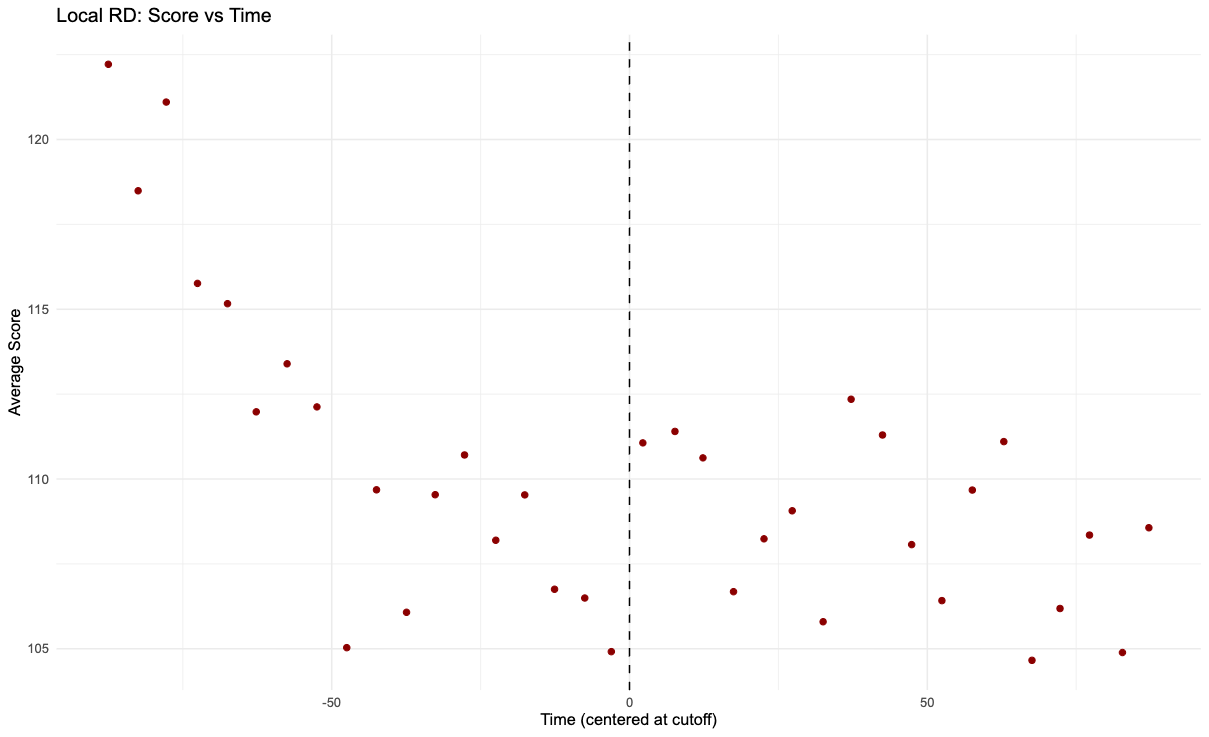
\includegraphics[width=0.8\textwidth]{figures/q1_1.png}
    \caption{Local RD plot 1}
    \label{fig:rd1_1}
\end{figure}

\begin{figure}[H]
    \centering
    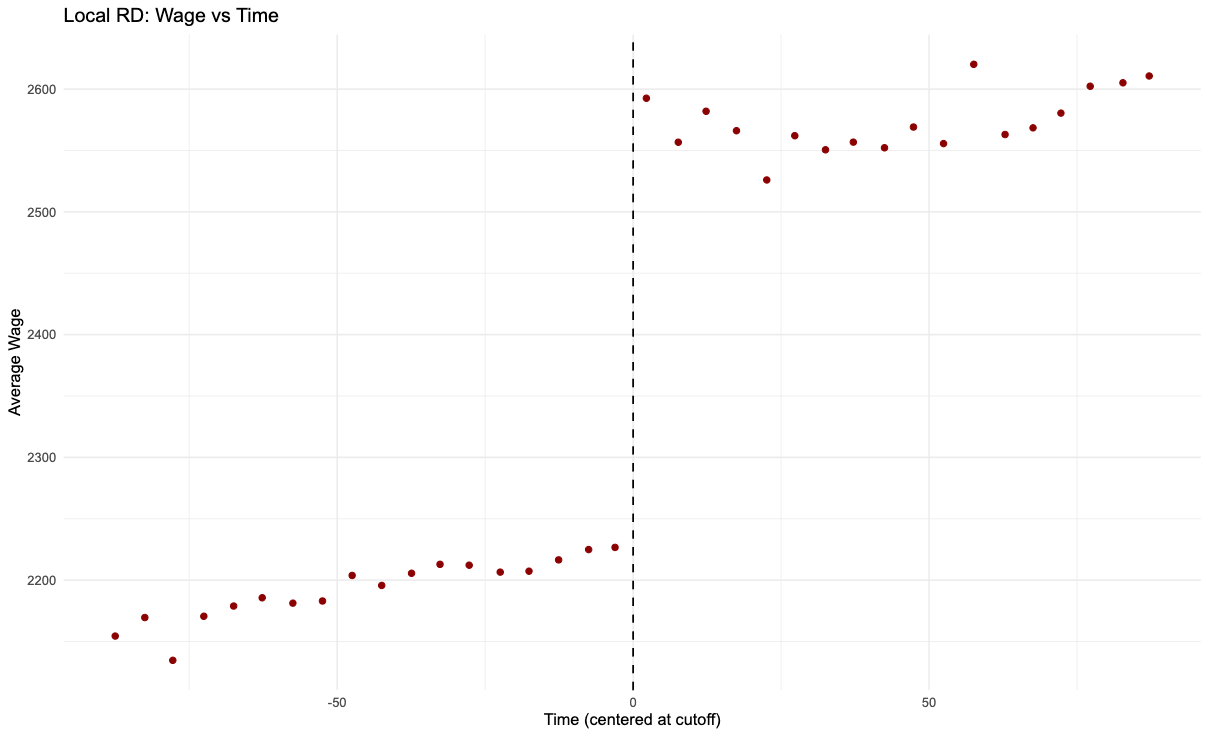
\includegraphics[width=0.8\textwidth]{figures/q1_2.png}
    \caption{Local RD plot 2}
    \label{fig:rd1_2}
\end{figure}

\begin{figure}[H]
    \centering
    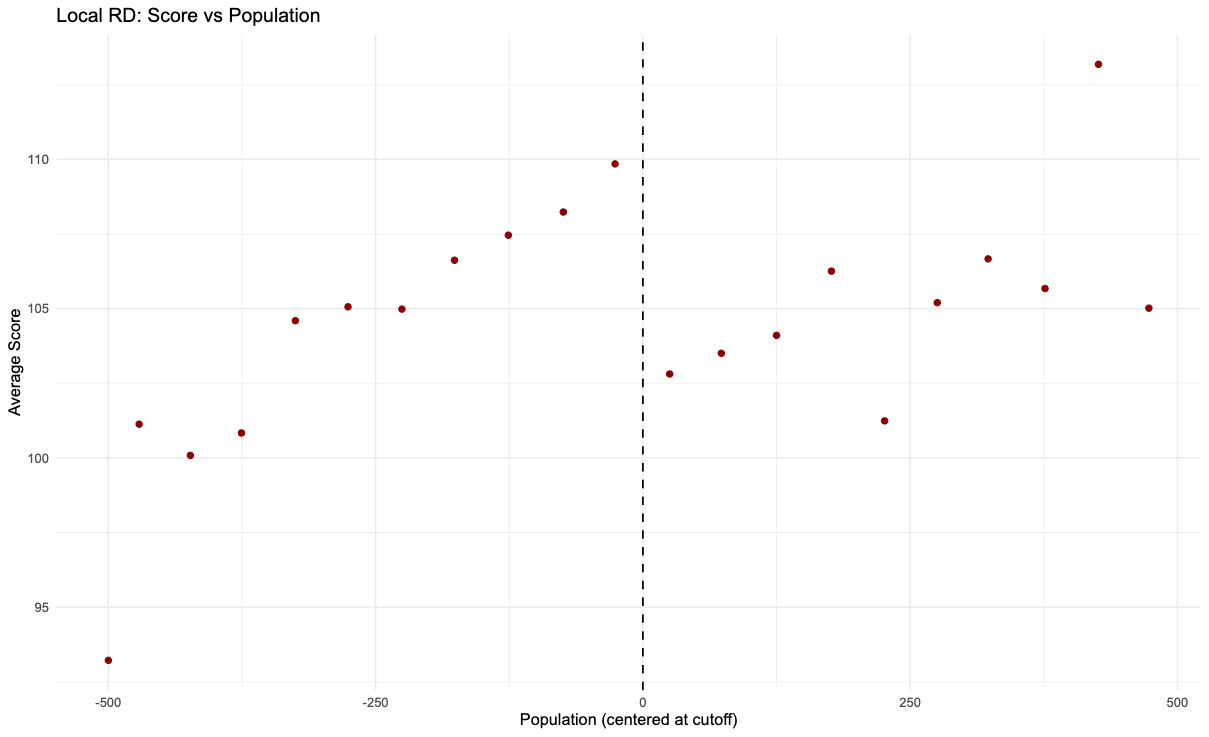
\includegraphics[width=0.8\textwidth]{figures/q1_3.png}
    \caption{Local RD plot 3}
    \label{fig:rd1_3}
\end{figure}


\begin{figure}[H]
    \centering
    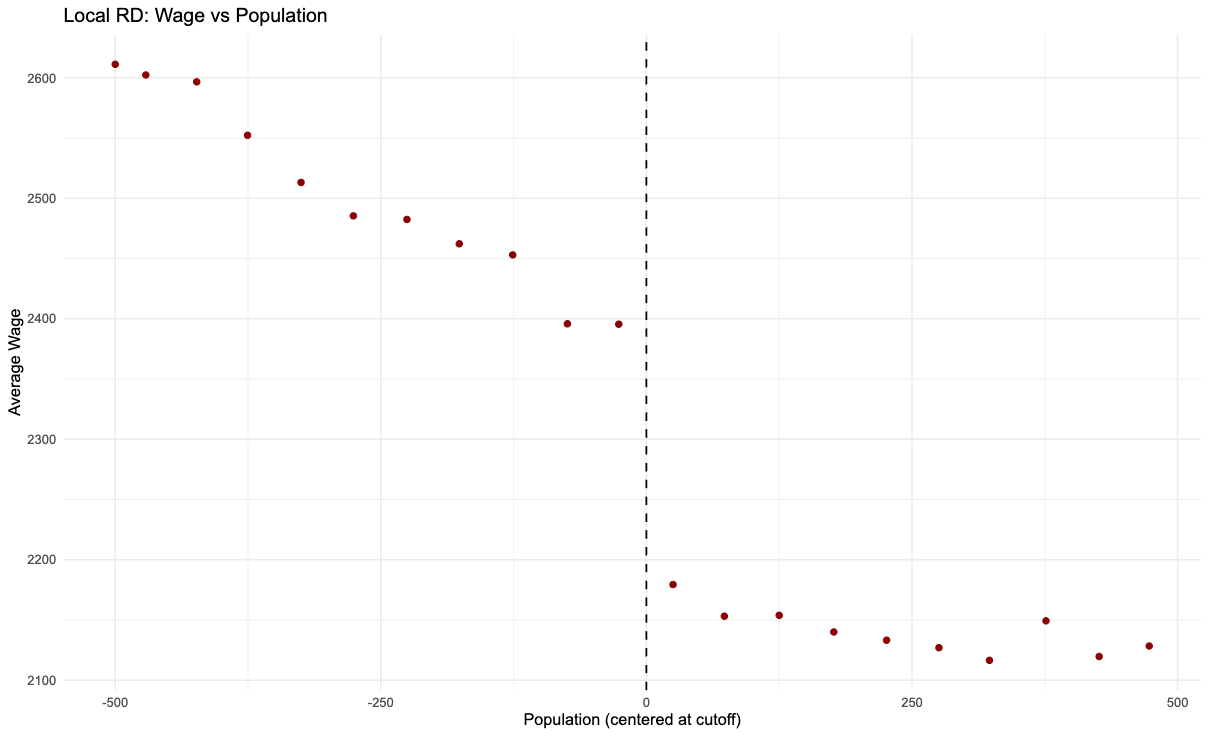
\includegraphics[width=0.8\textwidth]{figures/q1_4.png}
    \caption{Local RD plot 4}
    \label{fig:rd1_4}
\end{figure}

\begin{figure}[H]
    \centering
    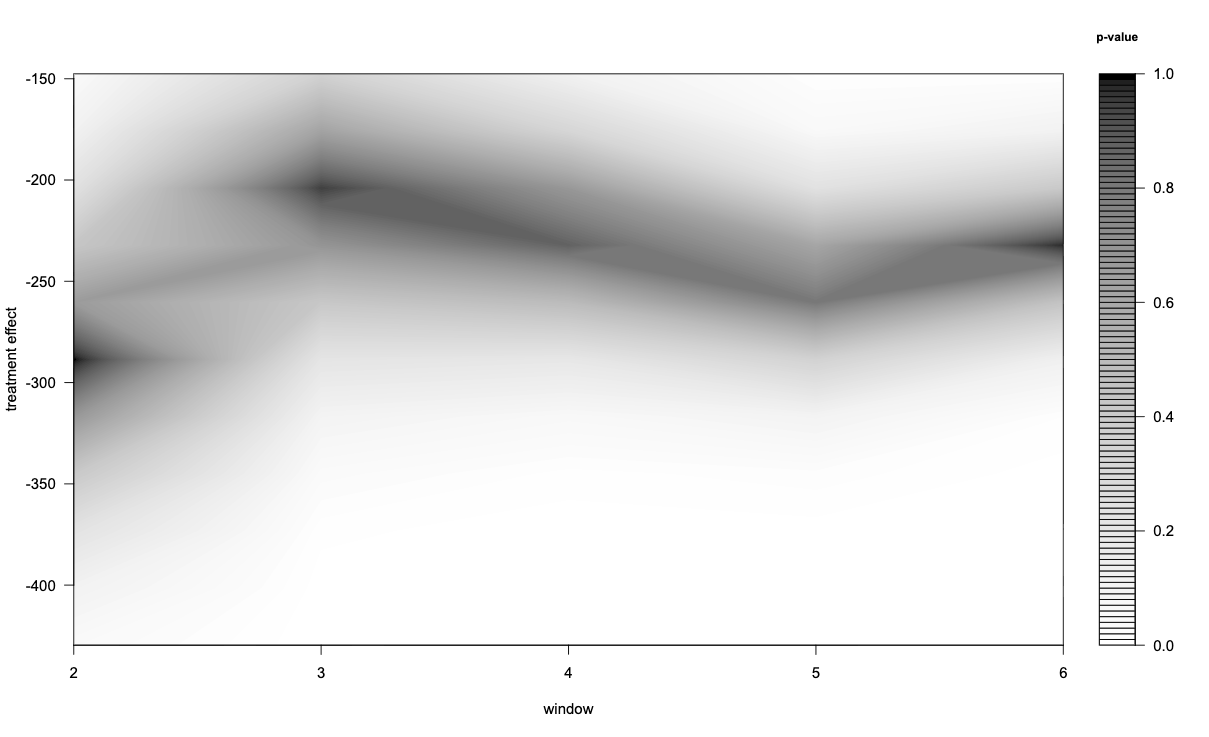
\includegraphics[width=0.8\textwidth]{figures/q1_sensitivity_1.png}
    \caption{Sensitivity analysis 1. Wage vs population}
    \label{fig:q1_sensitivity_1}
\end{figure}

\begin{figure}[H]
    \centering
    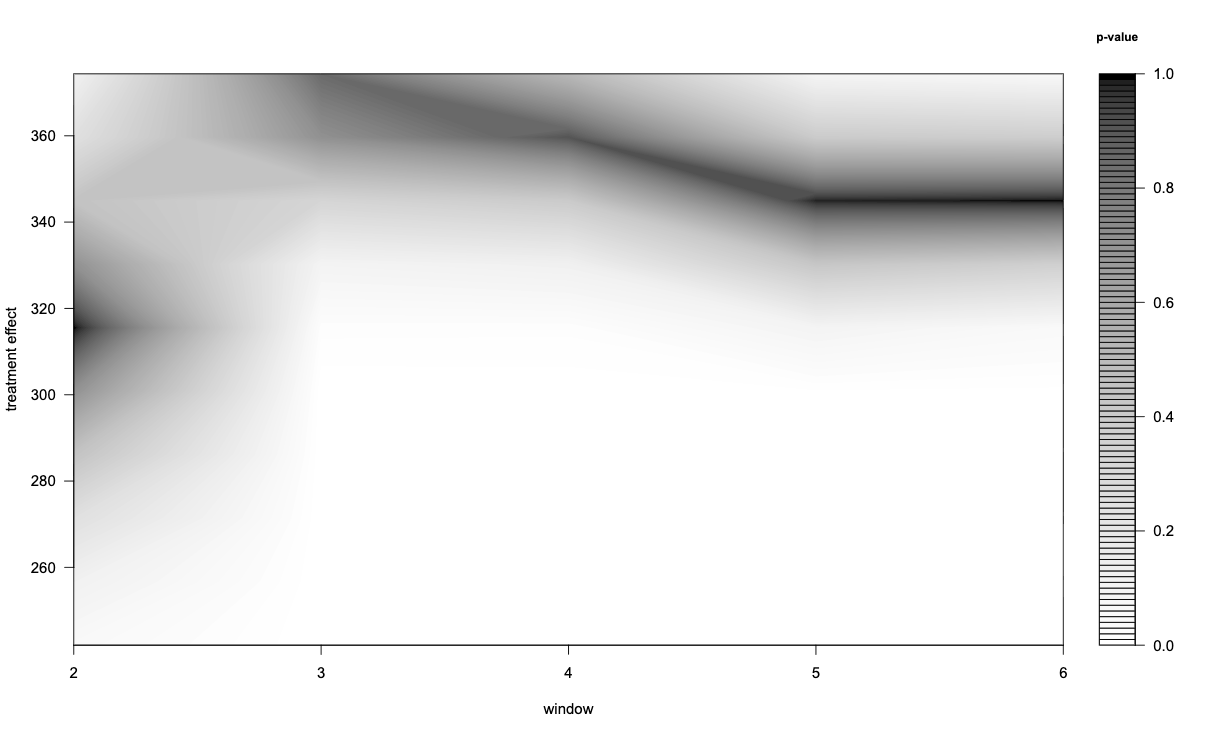
\includegraphics[width=0.8\textwidth]{figures/q1_sensitivity_2.png}
    \caption{Sensitivity analysis 2. Wage vs time}
    \label{fig:q1_sensitivity_2}
\end{figure}

\begin{figure}[H]
    \centering
    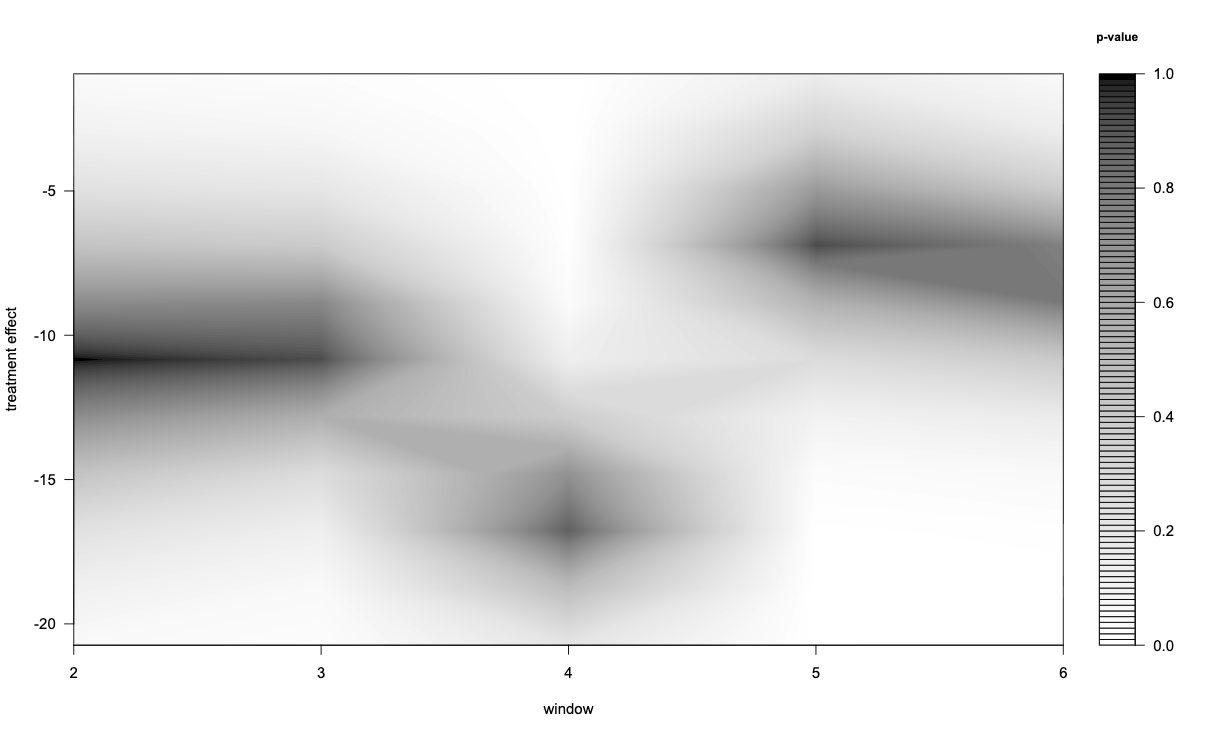
\includegraphics[width=0.8\textwidth]{figures/q1_sensitivity_3.png}
    \caption{Sensitivity analysis 3. Score vs population}
    \label{fig:q1_sensitivity_3}
\end{figure}

\begin{figure}[H]
    \centering
    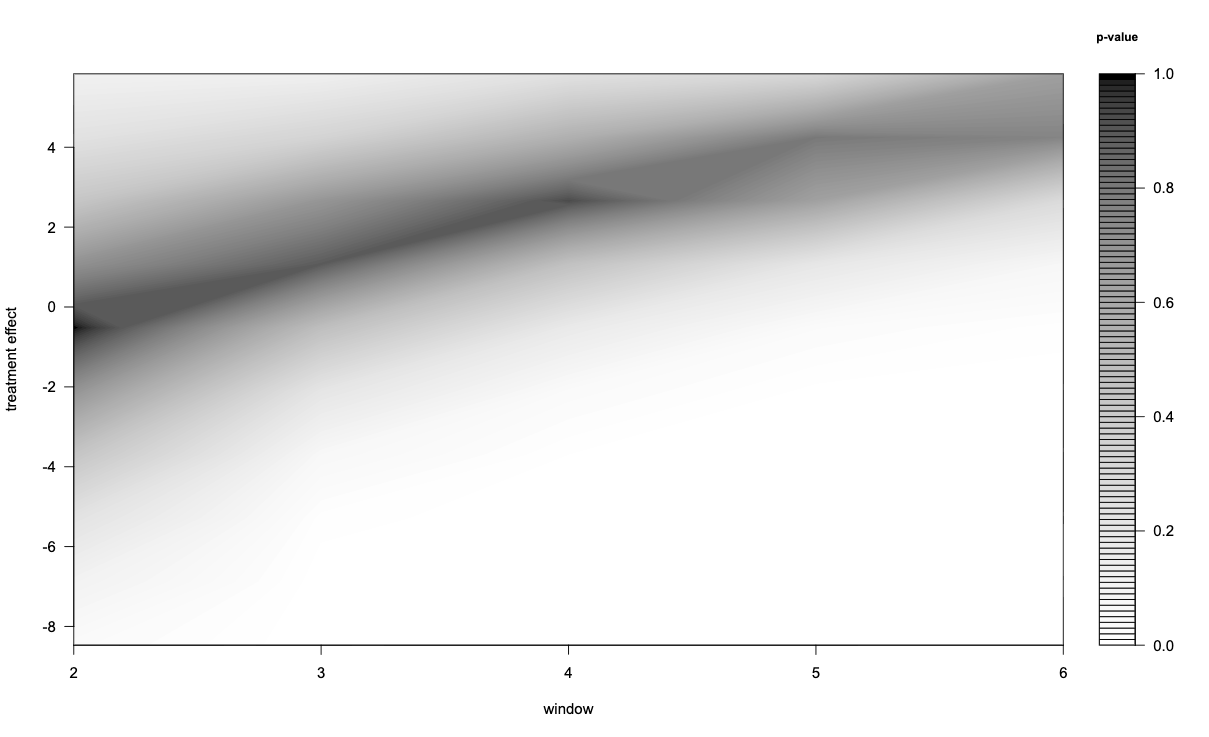
\includegraphics[width=0.8\textwidth]{figures/q1_sensitivity_4.png}
    \caption{Sensitivity analysis 4. Score vs time}
    \label{fig:q1_sensitivity_4}
\end{figure}

\begin{figure}[H]
    \centering
    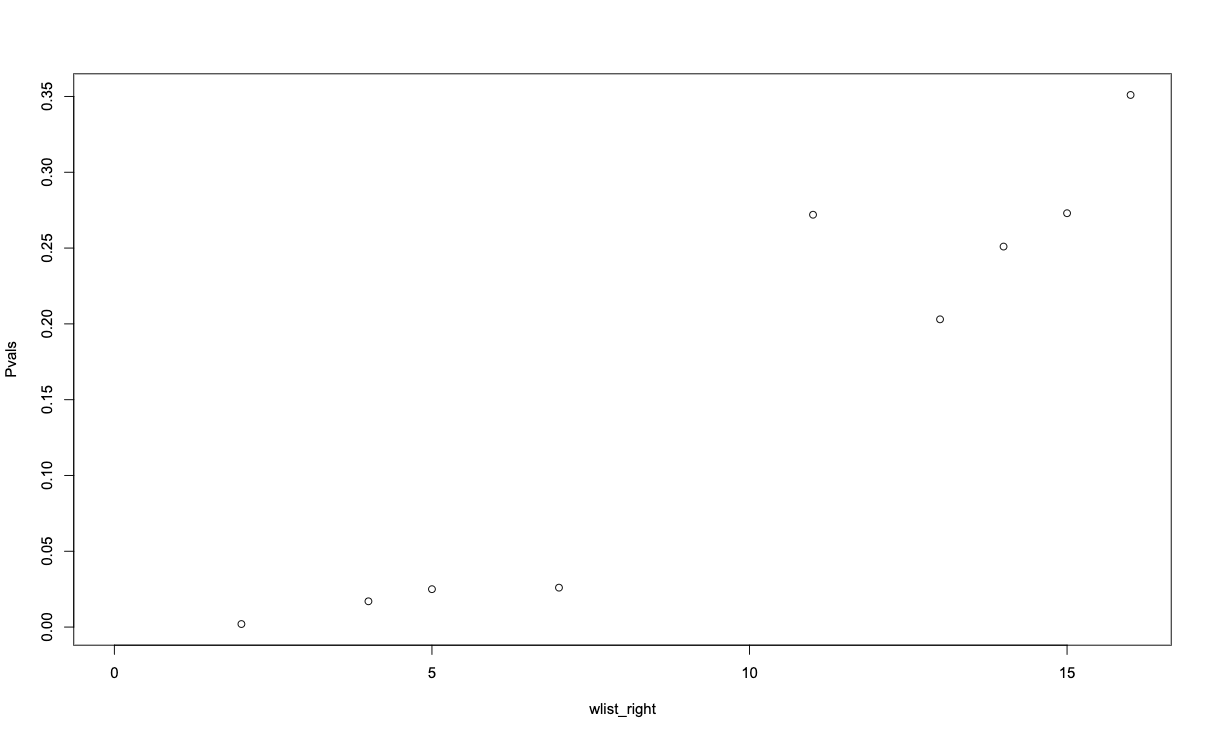
\includegraphics[width=0.8\textwidth]{figures/q1_pvalue1.png}
    \caption{P-value 1. Wage vs population}
    \label{fig:q1_pvalue_1}
\end{figure}

\begin{figure}[H]
    \centering
    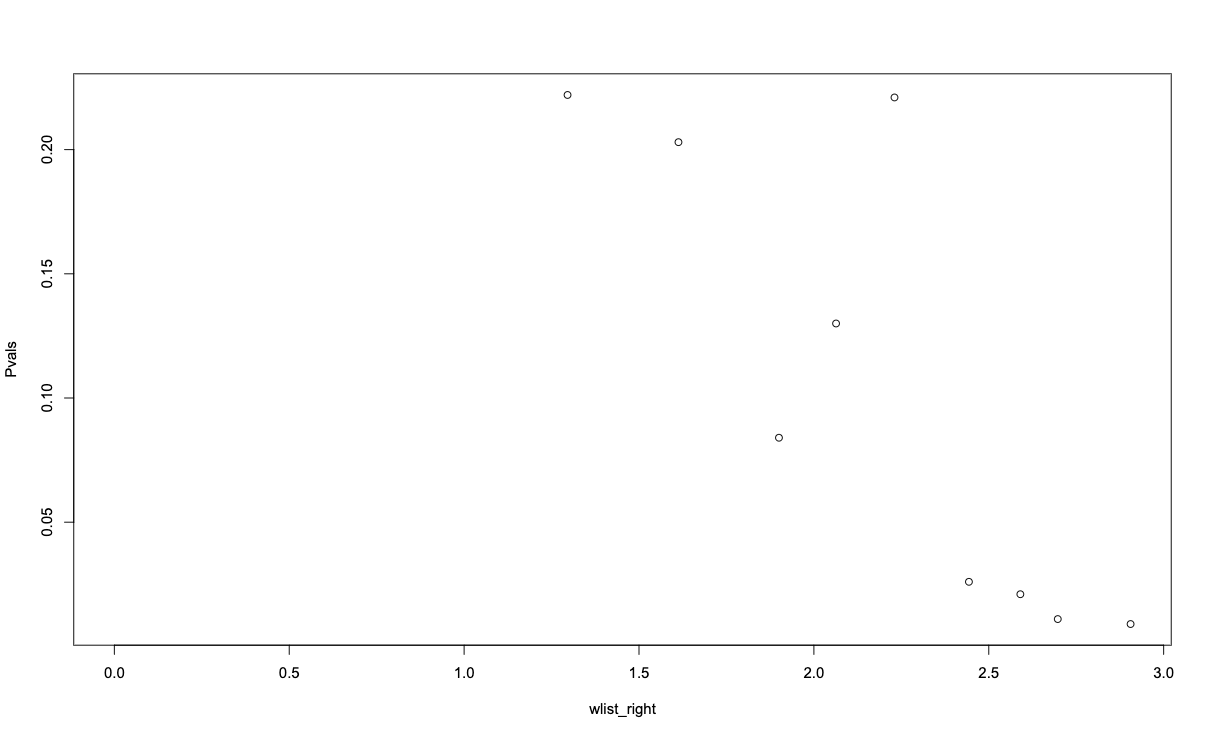
\includegraphics[width=0.8\textwidth]{figures/q1_pvalue2.png}
    \caption{P-value 2. Wage vs time}
    \label{fig:q1_pvalue_2}
\end{figure}

\begin{figure}[H]
    \centering
    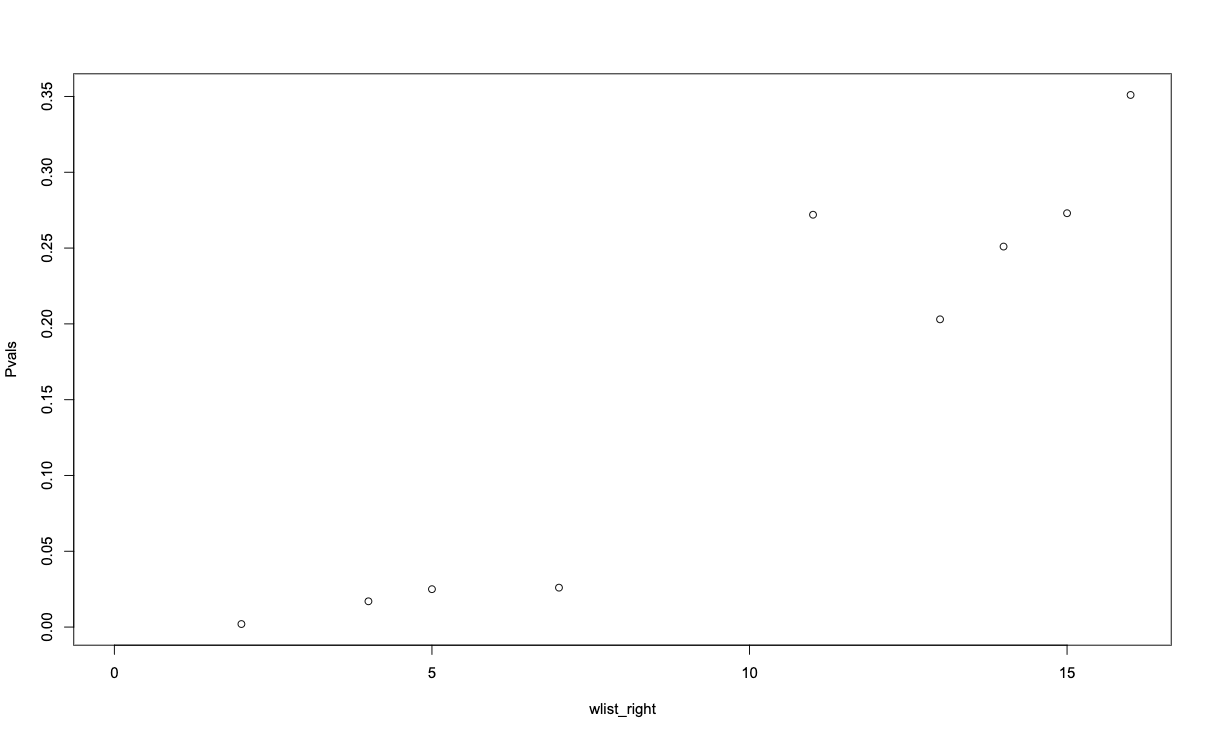
\includegraphics[width=0.8\textwidth]{figures/q1_pvalue3.png}
    \caption{P-value 3. Score vs population}
    \label{fig:q1_pvalue_3}
\end{figure}


\begin{figure}[H]
    \centering
    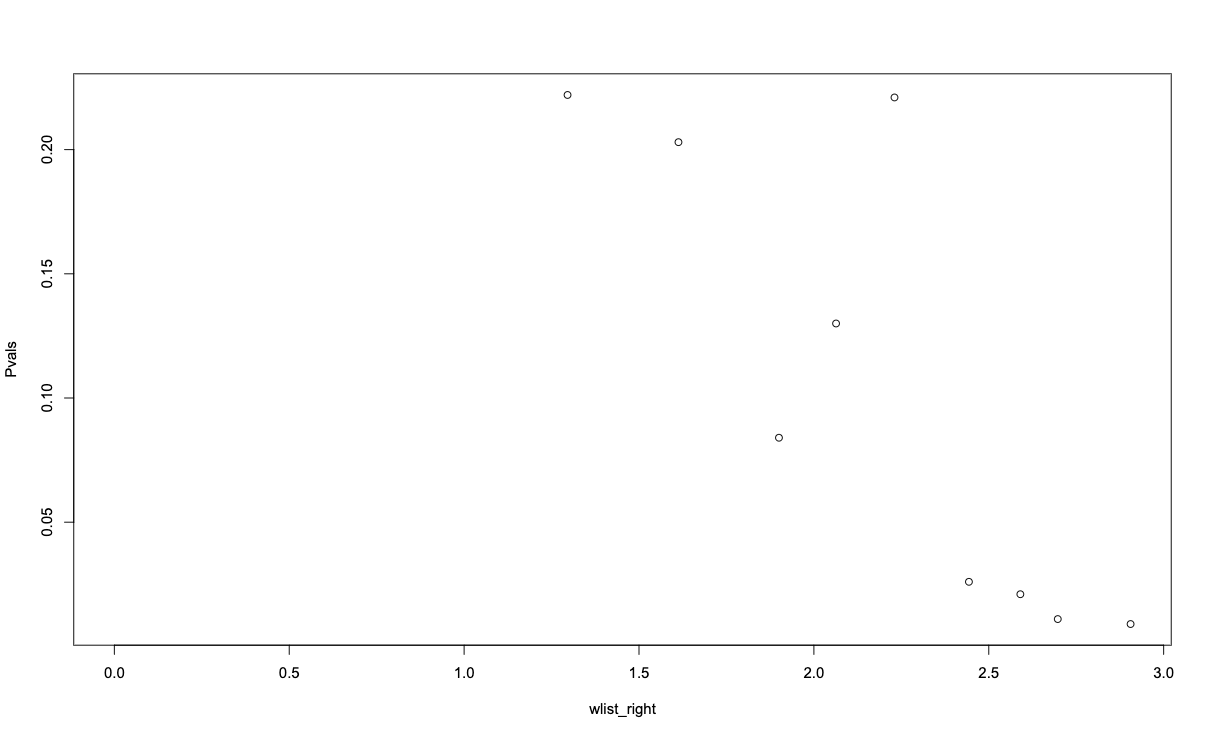
\includegraphics[width=0.8\textwidth]{figures/q1_pvalue4.png}
    \caption{P-value 4. Score vs time}
    \label{fig:q1_pvalue_4}
\end{figure}


\subsection*{Q.2}

\begin{figure}[H]
    \centering
    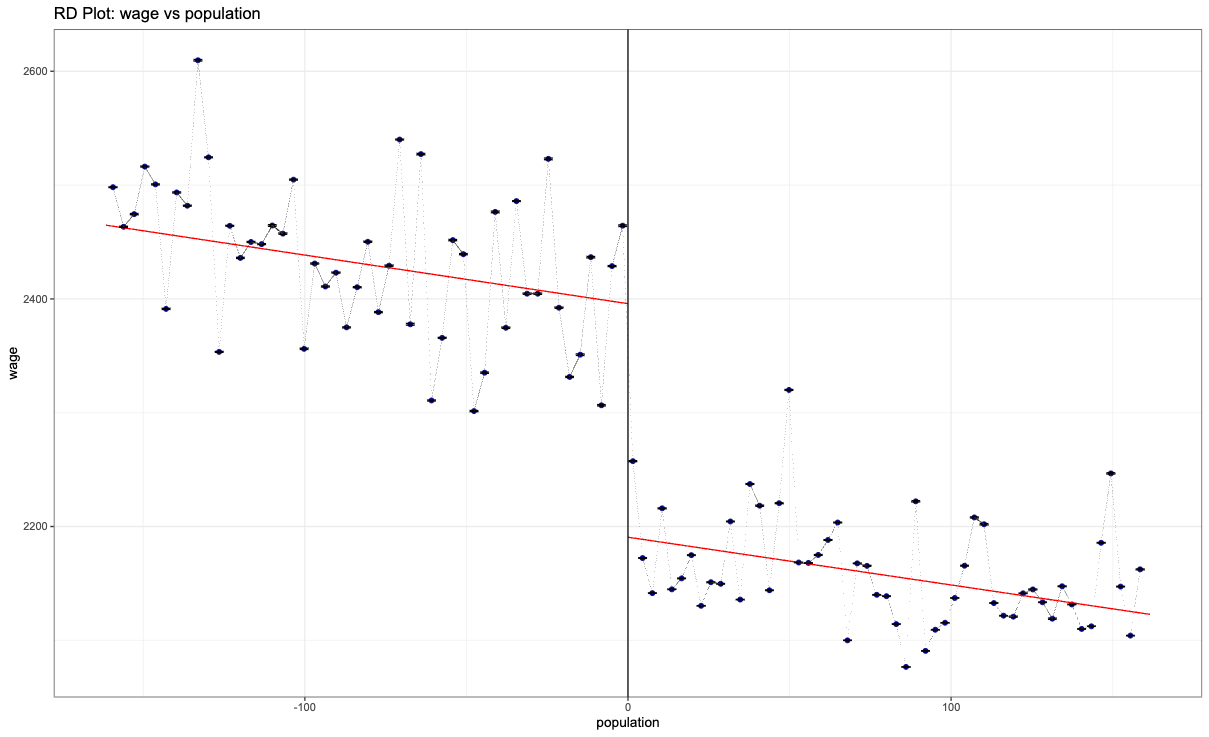
\includegraphics[width=0.8\textwidth]{figures/rd_cont_1.png}
    \caption{rdplot 1}
    \label{fig:rdcont1}
\end{figure}


\begin{figure}[H]
    \centering
    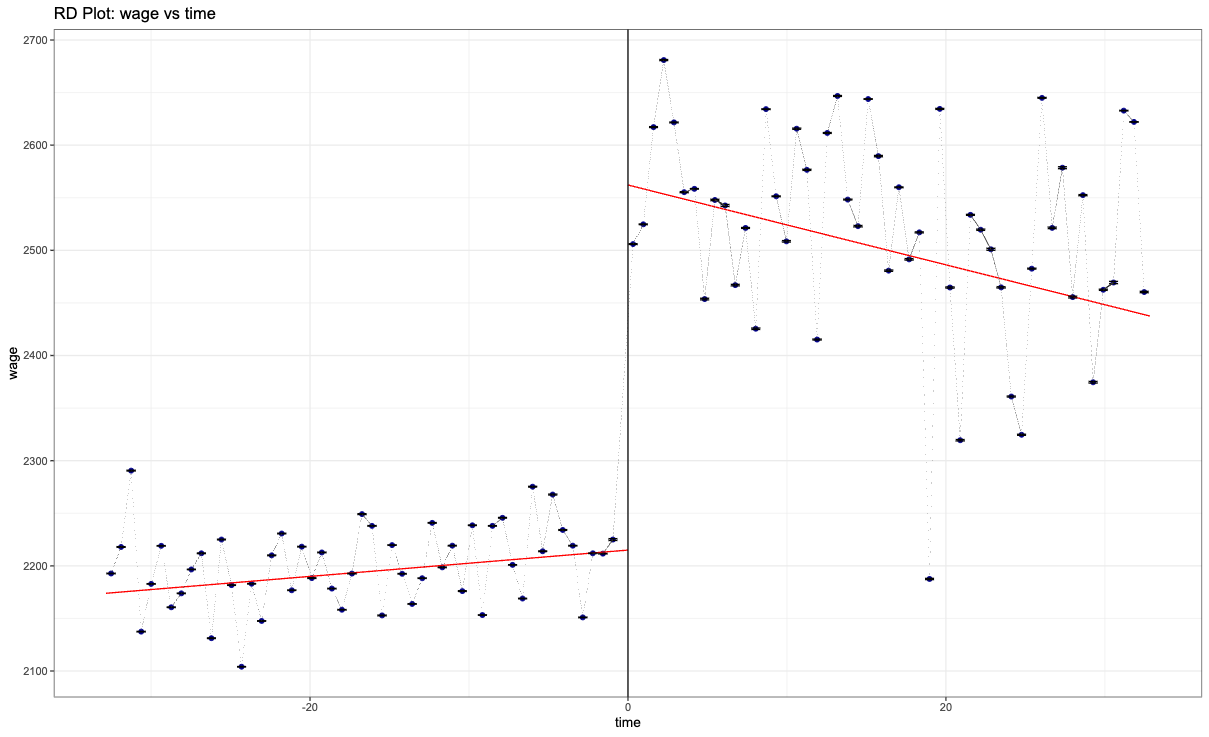
\includegraphics[width=0.8\textwidth]{figures/rd_cont_2.png}
    \caption{rdplot 2}
    \label{fig:rdcont2}
\end{figure}


\begin{figure}[H]
    \centering
    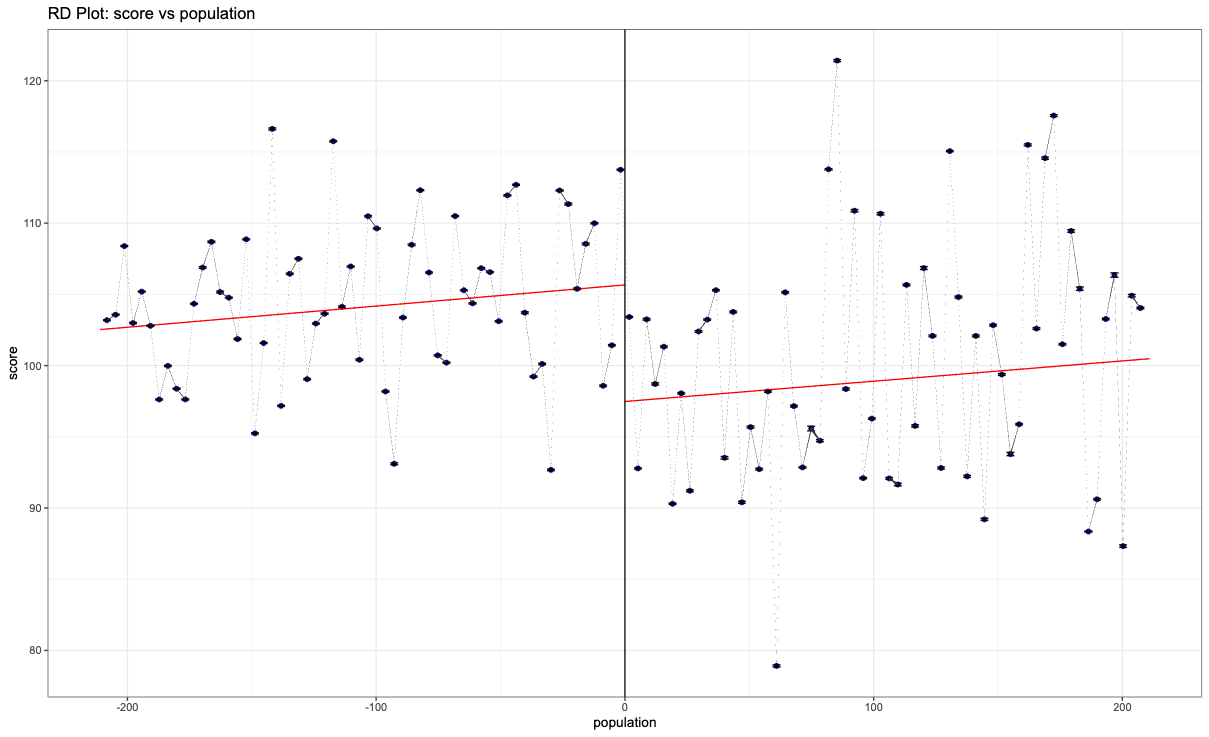
\includegraphics[width=0.8\textwidth]{figures/rd_cont_3.png}
    \caption{rdplot 3}
    \label{fig:rdcont3}
\end{figure}

\begin{figure}[H]
    \centering
    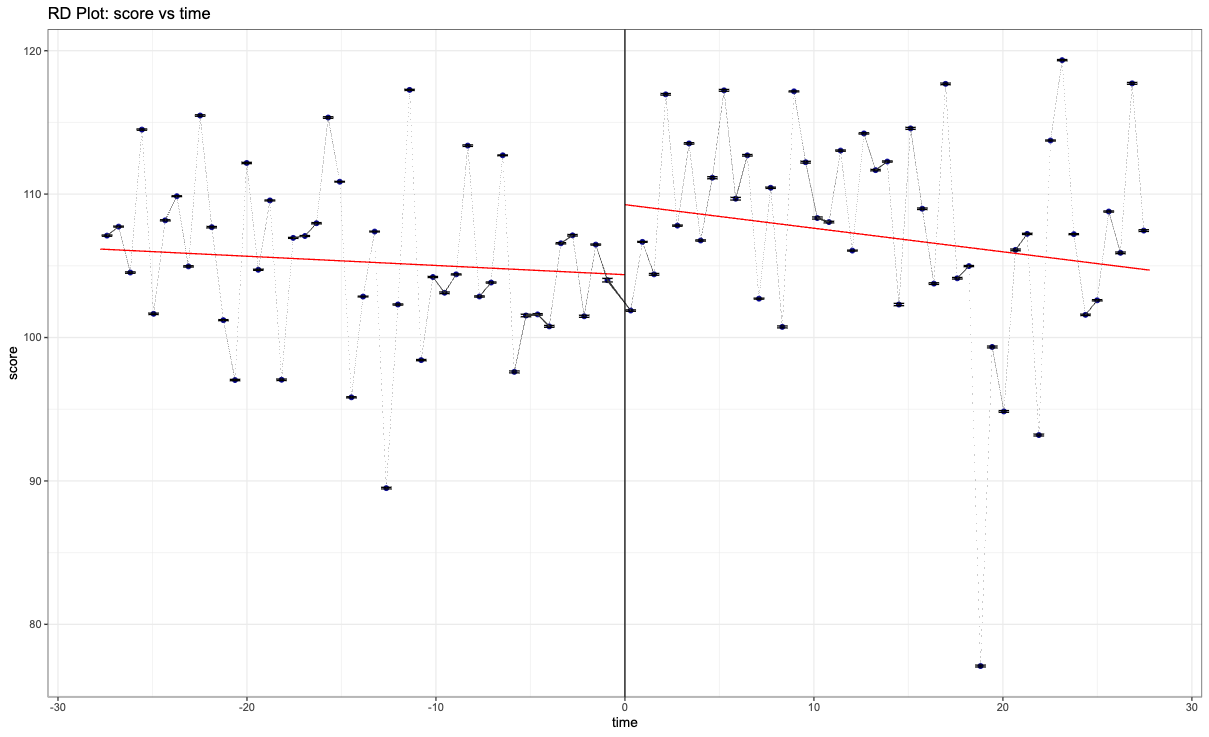
\includegraphics[width=0.8\textwidth]{figures/rd_cont_4.png}
    \caption{rdplot 4}
    \label{fig:rdcont4}
\end{figure}

\begin{figure}[H]
    \centering
    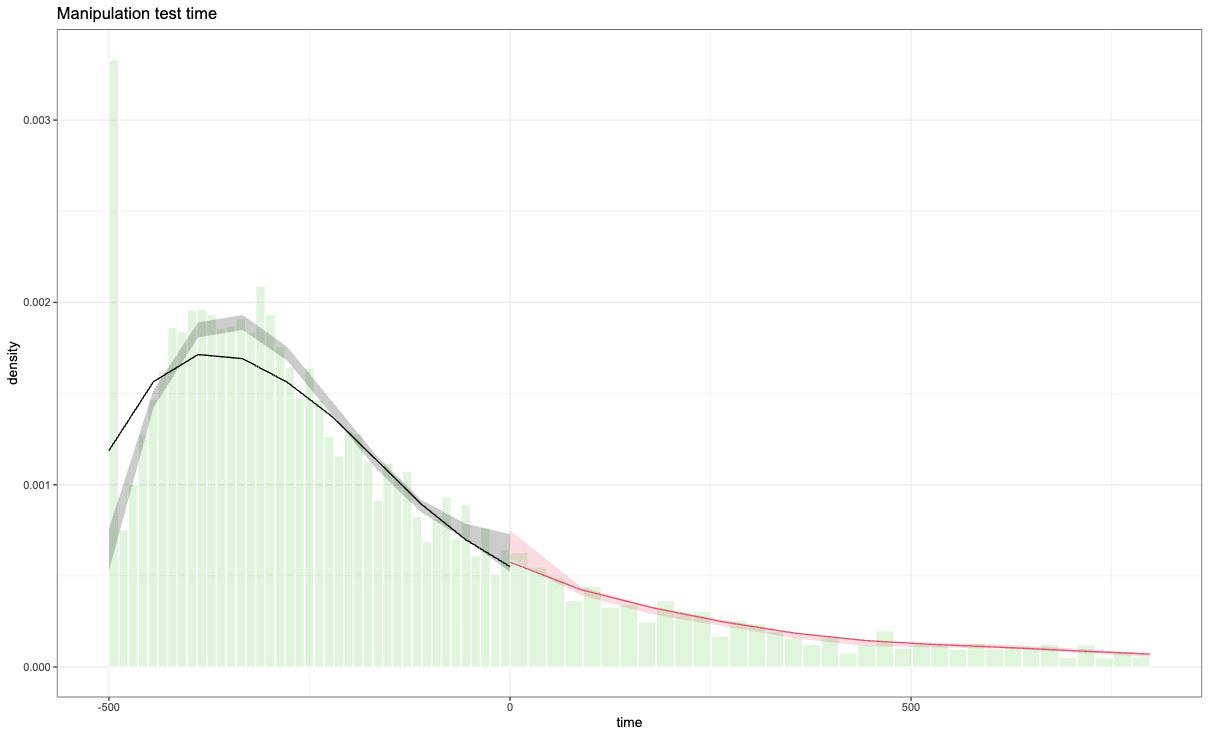
\includegraphics[width=0.8\textwidth]{figures/manipul_pop.png}
    \caption{manipulation test 1}
    \label{fig:manipul1}
\end{figure}

\begin{figure}[H]
    \centering
    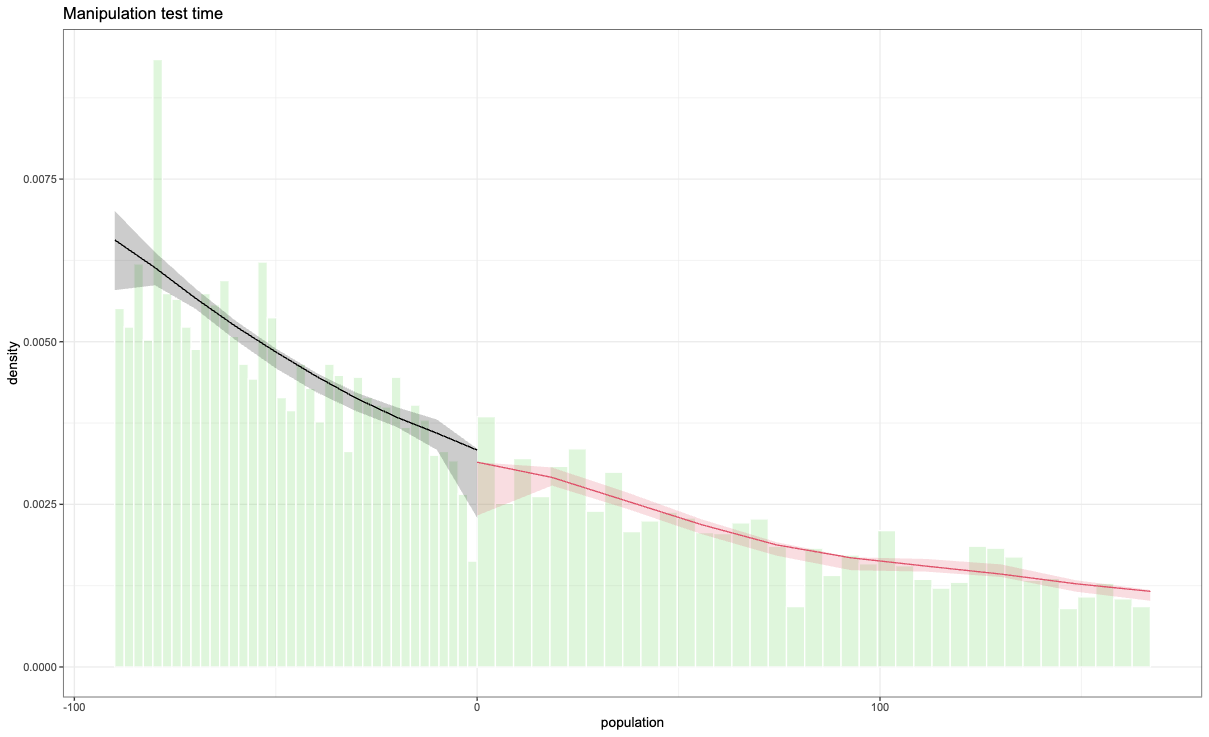
\includegraphics[width=0.8\textwidth]{figures/manipul_time.png}
    \caption{manipulation test 2}
    \label{fig:manipul2}
\end{figure}


\subsection*{Q.4}

\begin{figure}[H]
    \centering
    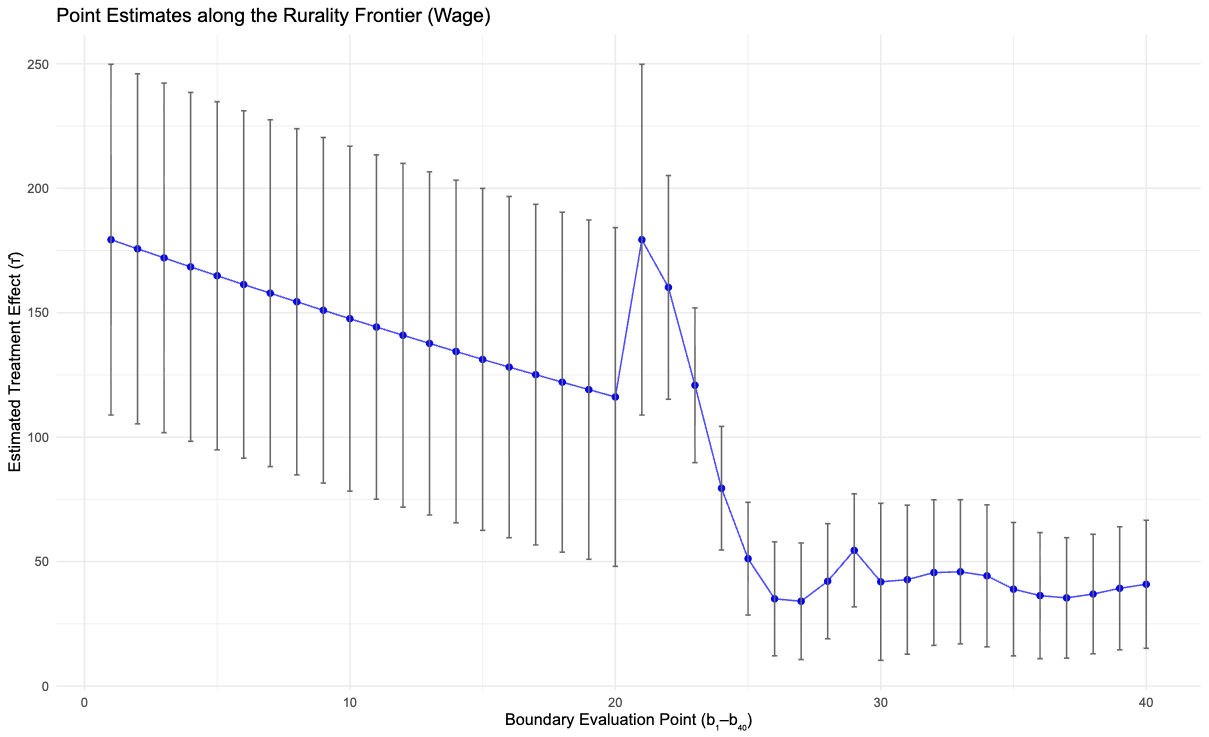
\includegraphics[width=0.8\textwidth]{figures/q4_1.png}
    \caption{boundary effects 1. Wage}
    \label{fig:boundary1}
\end{figure}

\begin{figure}[H]
    \centering
    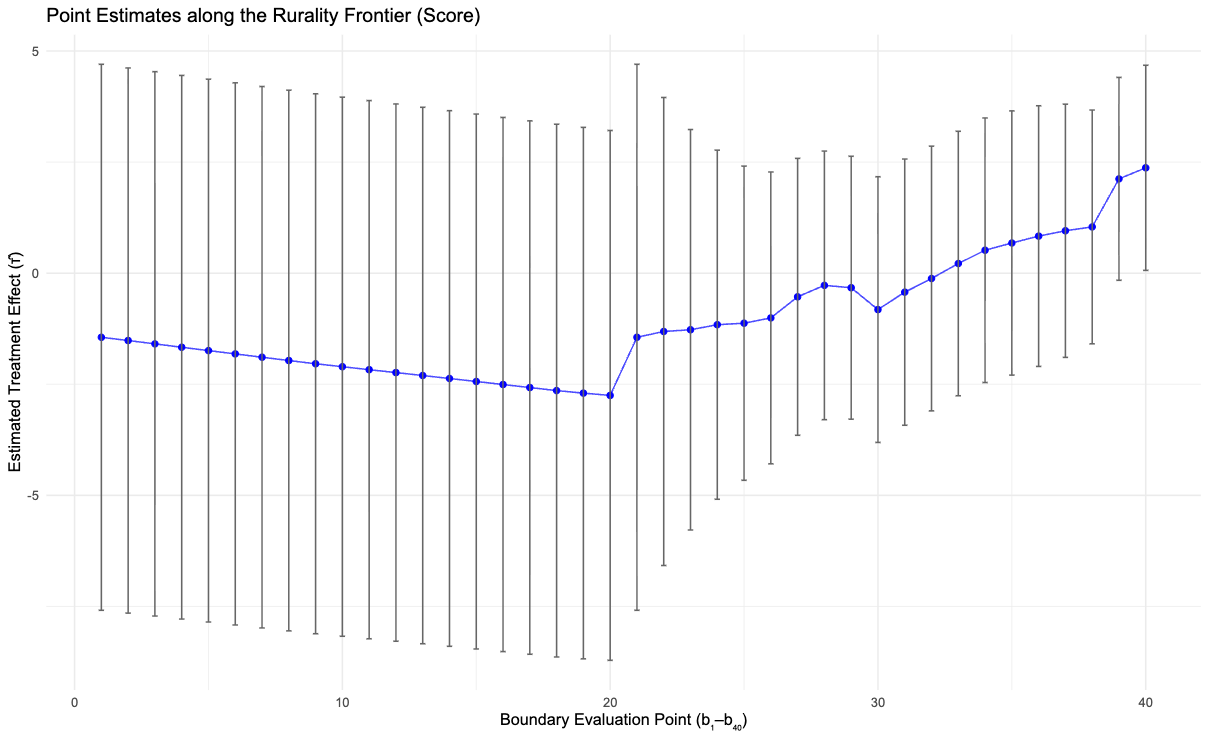
\includegraphics[width=0.8\textwidth]{figures/q4_2.png}
    \caption{boundary effects 2. Score}
    \label{fig:boundary2}
\end{figure}


\subsection*{Q.7}

\textbf{clogit}

\begin{figure}[H]
    \centering
    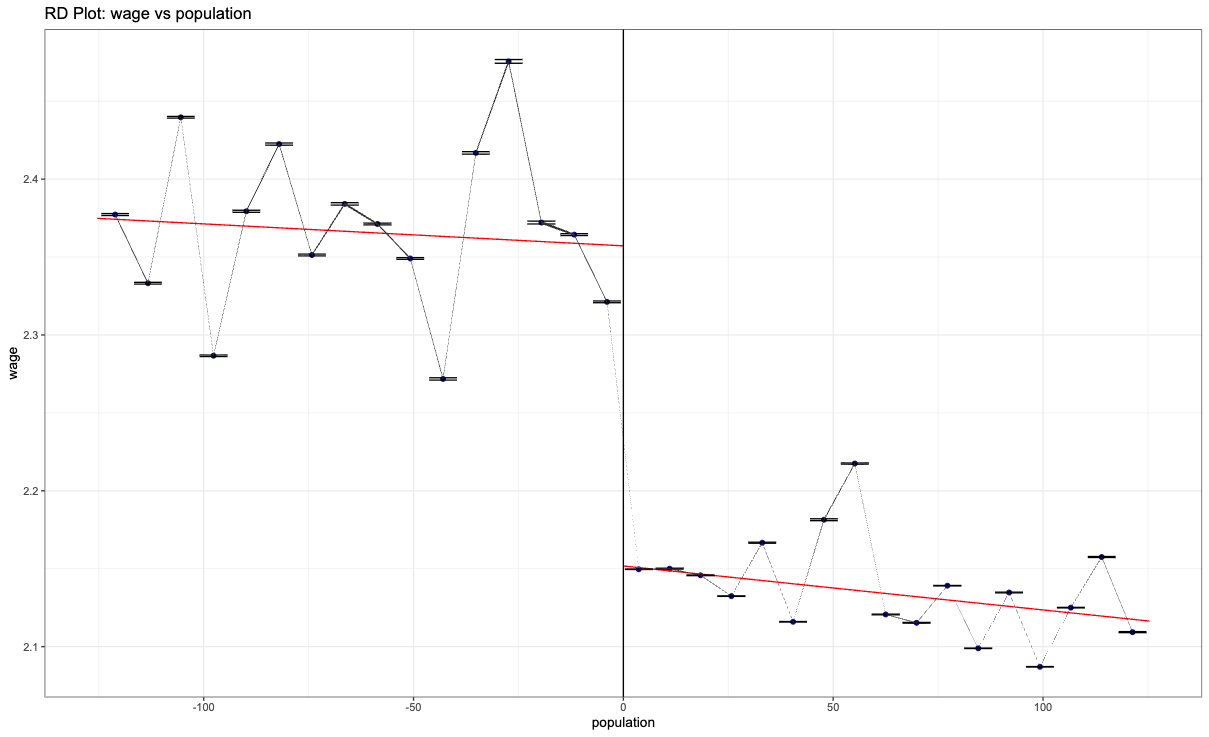
\includegraphics[width=0.8\textwidth]{figures/clogit_rd1.png}
    \caption{RD with clogit prediction}
    \label{fig:clogit_rd1}
\end{figure}

\begin{figure}[H]
    \centering
    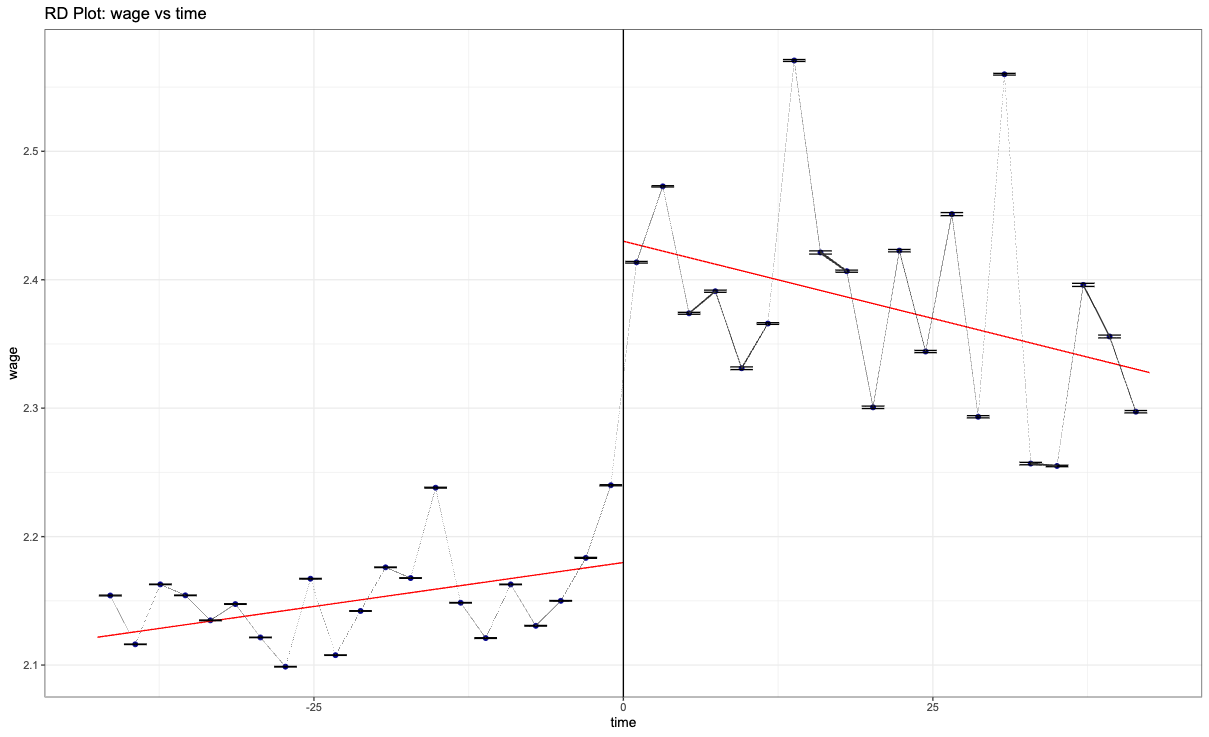
\includegraphics[width=0.8\textwidth]{figures/clogit_rd2.png}
    \caption{RD with clogit prediction}
    \label{fig:clogit_rd2}
\end{figure}

\begin{figure}[H]
    \centering
    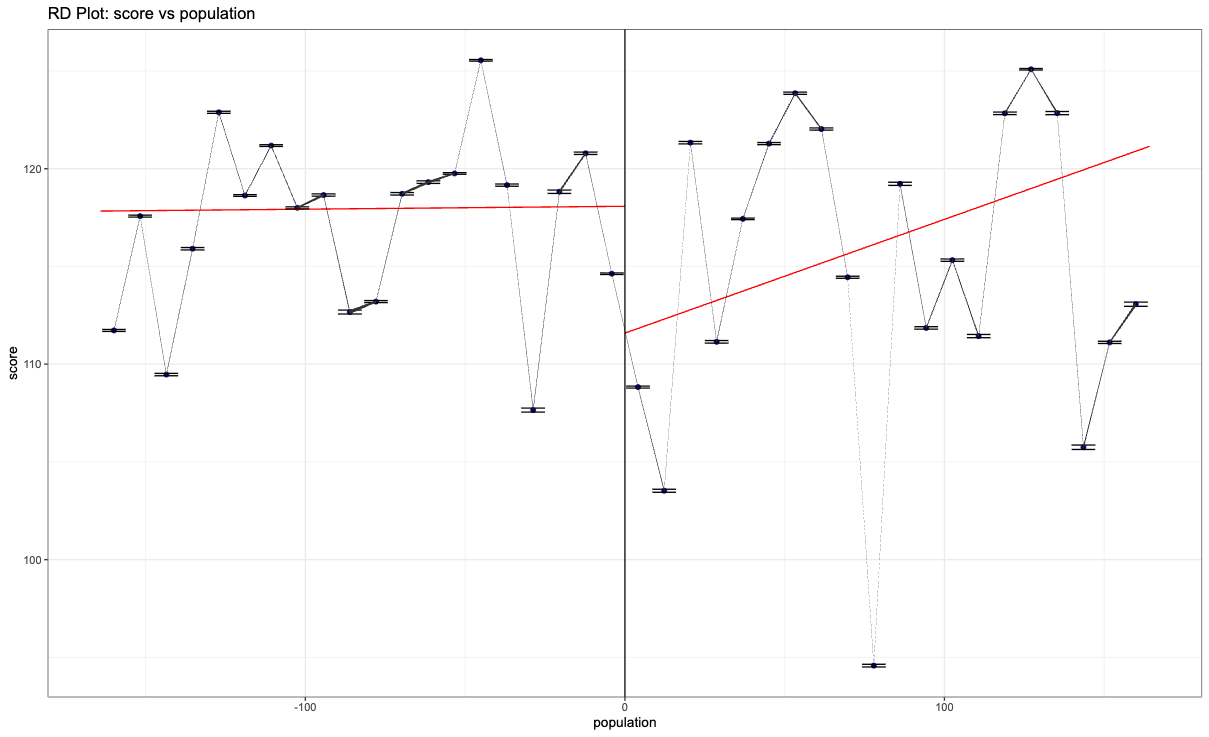
\includegraphics[width=0.8\textwidth]{figures/clogit_rd3.png}
    \caption{RD with clogit prediction}
    \label{fig:clogit_rd3}
\end{figure}

\begin{figure}[H]
    \centering
    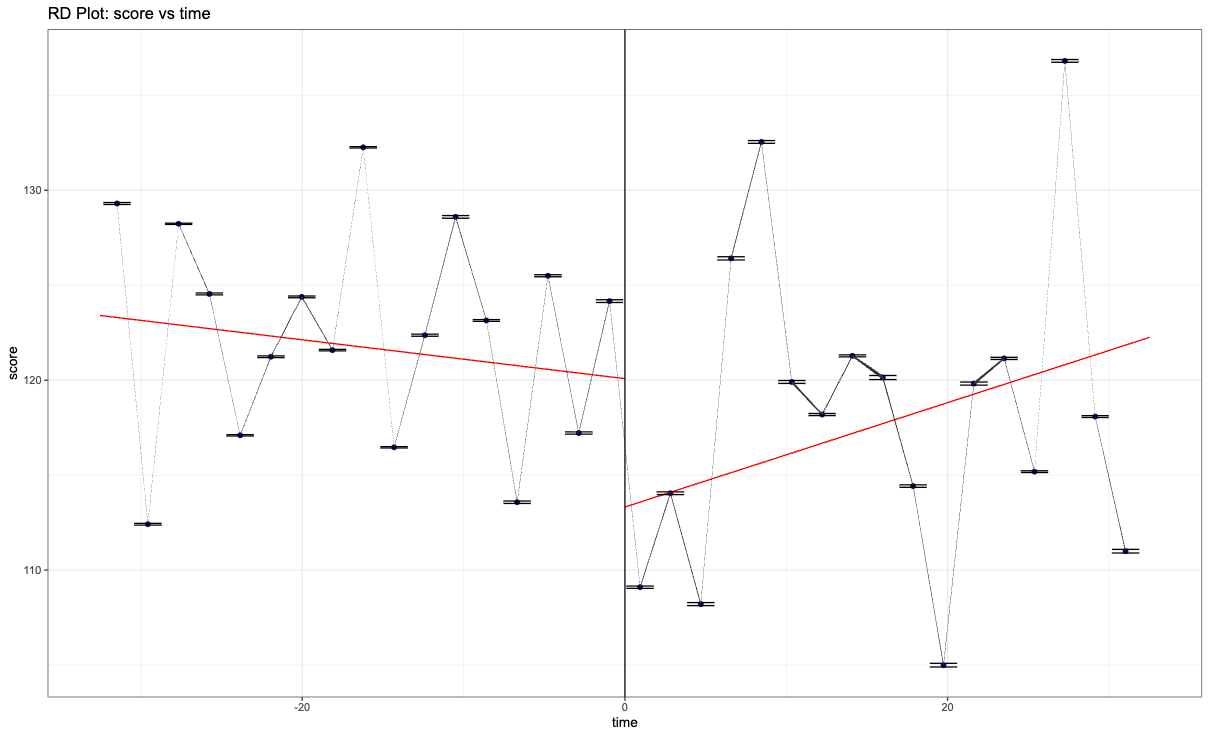
\includegraphics[width=0.8\textwidth]{figures/clogit_rd4.png}
    \caption{RD with clogit prediction}
    \label{fig:clogit_rd4}
\end{figure}

\textbf{mixlogit}

\begin{figure}[H]
    \centering
    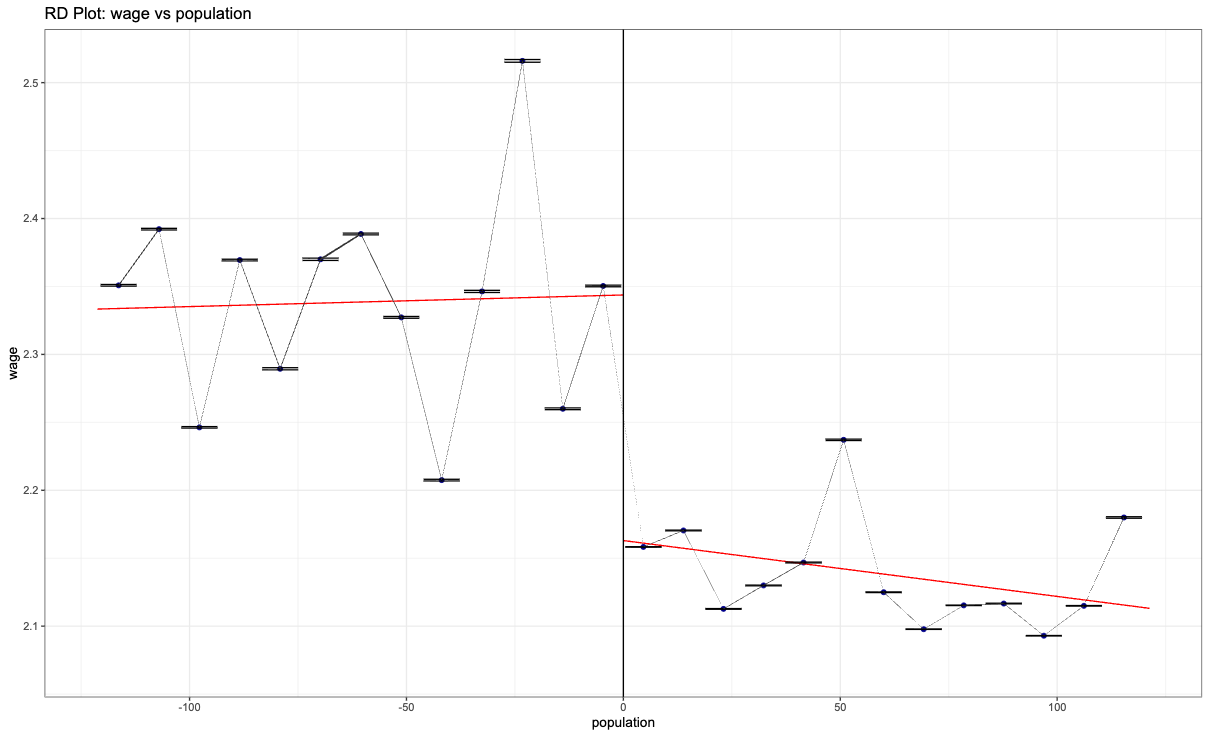
\includegraphics[width=0.8\textwidth]{figures/mixlogit_rd1.png}
    \caption{RD with clogit prediction}
    \label{fig:mixlogit_rd1}
\end{figure}

\begin{figure}[H]
    \centering
    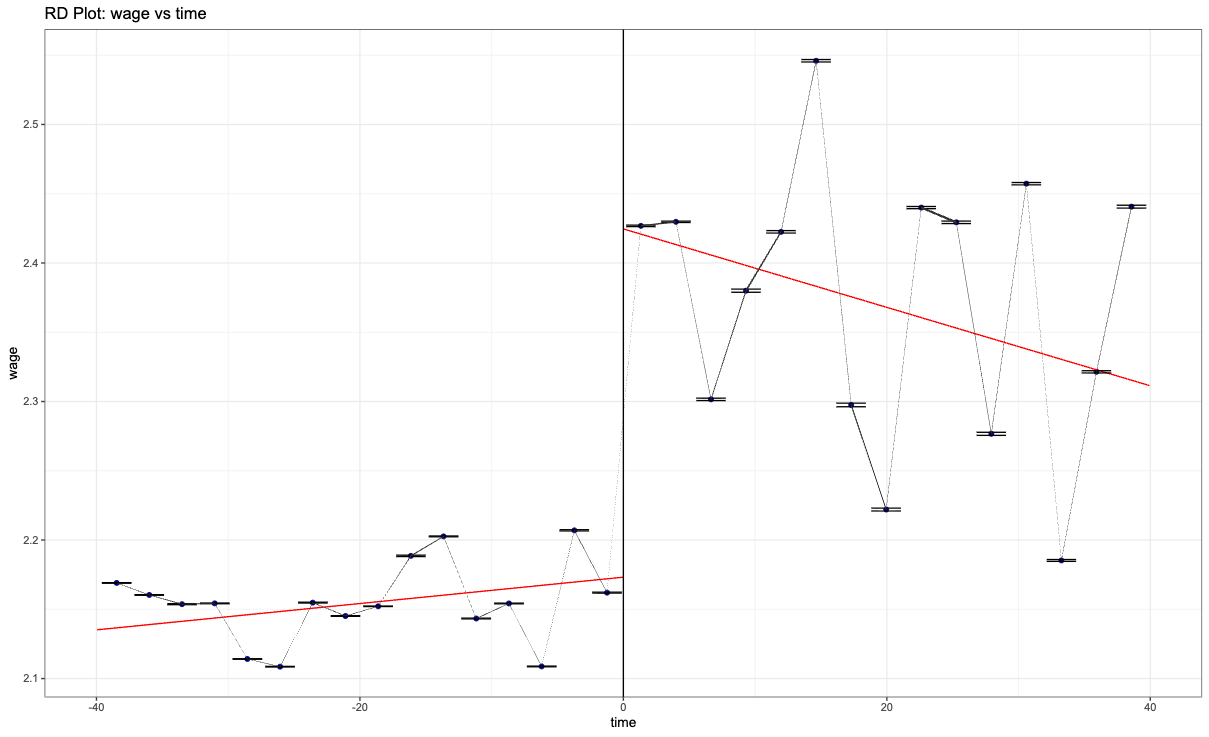
\includegraphics[width=0.8\textwidth]{figures/mixlogit_rd2.png}
    \caption{RD with clogit prediction}
    \label{fig:mixlogit_rd2}
\end{figure}

\begin{figure}[H]
    \centering
    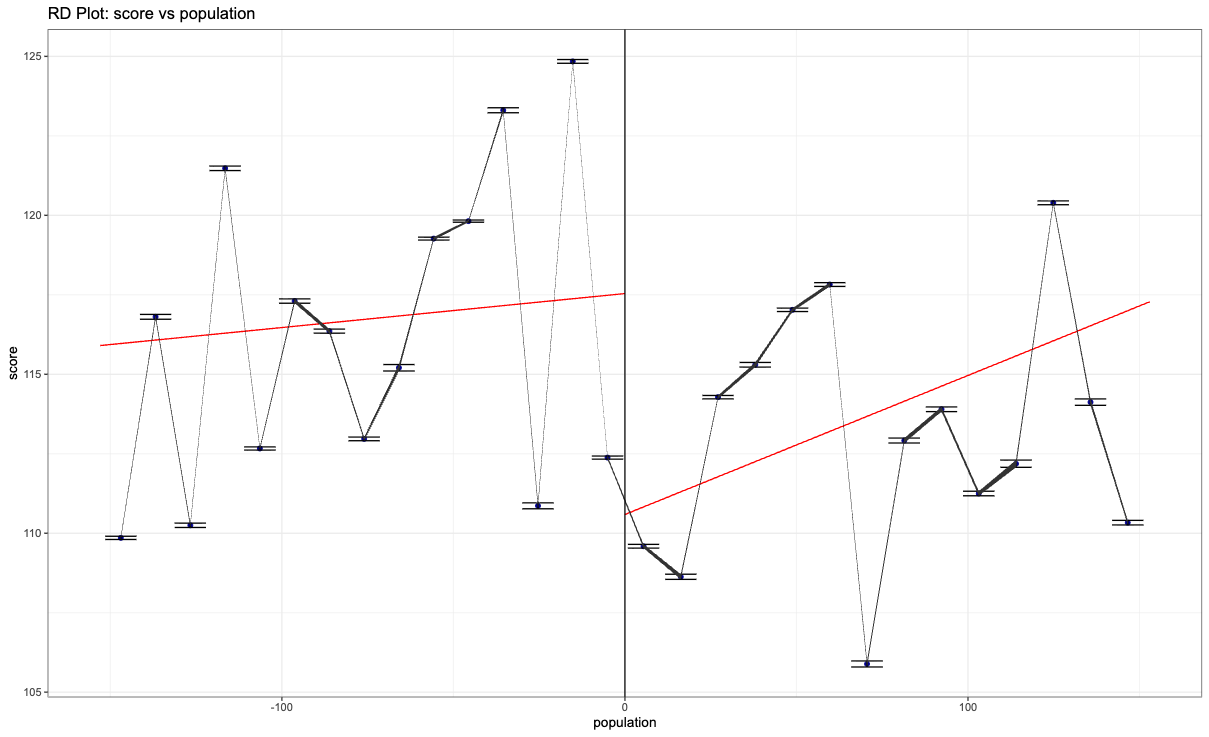
\includegraphics[width=0.8\textwidth]{figures/mixlogit_rd3.png}
    \caption{RD with clogit prediction}
    \label{fig:mixlogit_rd3}
\end{figure}

\begin{figure}[H]
    \centering
    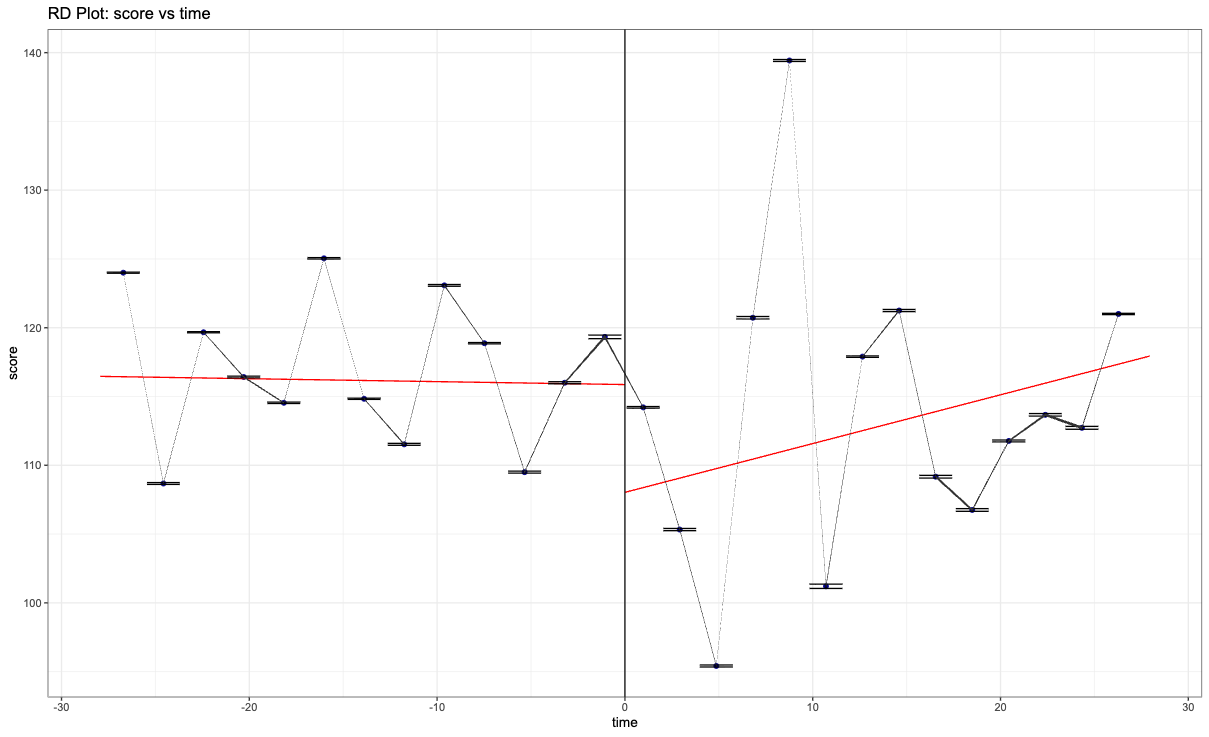
\includegraphics[width=0.8\textwidth]{figures/mixlogit_rd4.png}
    \caption{RD with clogit prediction}
    \label{fig:mixlogit_rd4}
\end{figure}

\end{document}


